% ============================================================
% GLOBAL SETTINGS: edit these values to change layout
%   Font size         : change the class option below (10pt / 11pt / 12pt)
%   Body line spacing : change \reportlinespacing (1.0 = single, 1.5, 2.0 = double)
%   Title/TOC spacing : change \reporttitlelinespacing (applied only to title page and TOC)
% ============================================================
\documentclass[12pt, letterpaper]{article}   % <-- font size set here

% ----- Packages -----
\usepackage[utf8]{inputenc}
\usepackage[top=1.25in, bottom=1.25in, left=1.0in, right=1.0in]{geometry}
\usepackage{graphicx}              % For including images/logos
\usepackage{xcolor}                % For custom colors (ASU red)
\usepackage{hyperref}              % For clickable TOC and links
\usepackage{tabularx}              % For dynamic width tables
\usepackage{parskip}               % Adds space between paragraphs (no indentation)
\usepackage{fancyhdr}              % For page numbers
\usepackage{helvet}                % Sans-serif font similar to the original document
\usepackage{lipsum}                % FOR PLACEHOLDER TEXT (Lorem Ipsum)
\usepackage{amsmath}               % For \text command in math mode
\usepackage{amssymb}               % For \mathbb command (math blackboard bold)
\usepackage{float}                 % For precise figure placement
\usepackage{microtype}             % Micro-typography to prevent overfull lines
\usepackage{setspace}              % For line spacing control
\usepackage{titlesec}              % For section/subsection title formatting
\setlength{\emergencystretch}{3em} % Allow extra stretch to avoid margin overflow
\renewcommand{\familydefault}{\sfdefault}

\def\reportlinespacing{1.5}        % <-- body line spacing set here
\def\reporttitlelinespacing{1.0}   % <-- title page & TOC line spacing set here
\setstretch{\reportlinespacing}

% ----- Section/Subsection Title Formatting -----
\titleformat{\section}{\fontsize{14}{17}\selectfont\bfseries}{\thesection}{1em}{}
\titleformat{\subsection}{\fontsize{12}{15}\selectfont\bfseries}{\thesubsection}{1em}{}
\titleformat{\subsubsection}{\fontsize{12}{15}\selectfont\bfseries}{\thesubsubsection}{1em}{}
\titlespacing*{\section}{0pt}{2.0in}{0.5em}
\titlespacing*{\subsection}{0pt}{1em}{0.5em}
\titlespacing*{\subsubsection}{0pt}{1em}{0.5em}

% ----- Page Setup -----
\pagestyle{fancy}
\fancyhf{} % Clear all header and footer fields
\renewcommand{\headrulewidth}{0pt} % Remove top header line
\fancyfoot[R]{\thepage} % Page number on the bottom right
\fancypagestyle{plain}{% Override plain style (used by title, TOC, etc.)
  \fancyhf{}%
  \renewcommand{\headrulewidth}{0pt}%
  \fancyfoot[R]{\thepage}%
}

% Define ASU Maroon Color (Approximate)
\definecolor{asumaroon}{RGB}{140, 29, 64}

% Link colors for TOC
\hypersetup{
    colorlinks=true,
    linkcolor=black,
    citecolor=blue,
    filecolor=magenta,      
    urlcolor=blue,
}
\setcounter{tocdepth}{3}

\begin{document}

% ==========================================
% TITLE PAGE
% ==========================================
\begin{titlepage}
    \setstretch{\reporttitlelinespacing}
    \thispagestyle{fancy}
    
    \begin{center}
        \vspace*{1cm}
        
        % Inserted the ASU Logo
        
\includegraphics[width=0.6\textwidth]{ASU-logo.png} 
        
        \vspace{1cm}
        
        {\normalsize\textbf{CSE 543: Information Assurance \& Security} \par}

        \vspace{1cm}

        \hrule

        \vspace{1cm}

        {\normalsize\textbf{Detection of Prompt Injection Attacks in LLM-Based Software Services Using Supervised Machine Learning} \par}

        \vspace{0.2cm}

        {\normalsize\textbf{Group 9 - Course Project Report} \par}
        
    \end{center}
    
    \vspace{1cm}
    
    \noindent List of Team Members:
    
    \vspace{0.5cm}
    
    \renewcommand{\arraystretch}{1.5}
    \noindent
    \begin{tabularx}{\textwidth}{|c|X|X|l|}
        \hline
        \multicolumn{1}{|c|}{ASU ID} & \multicolumn{1}{c|}{NAME} & \multicolumn{1}{c|}{EMAIL ID} & \multicolumn{1}{c|}{ROLE} \\ \hline
        1237028938 & Maulik Jadav & mjadav@asu.edu & Leader \\ \hline
        1223975389 & Josie Lorenz & jaloren4@asu.edu & Member \\ \hline
        1237124618 & Vatsal Nirmal & vnirmal3@asu.edu & Deputy Leader \\ \hline
        1236767989 & Tawanda Nyagumbo & ttawanda@asu.edu & Member \\ \hline
        1238334320 & Shivasmaran Rajashekar & srajash9@asu.edu & Member \\ \hline
        1236446681 & Mohammad Jani Basha Shaik & mshaik68@asu.edu & Member \\ \hline
        1237522730 & Anish Paul Singareddy & asingar5@asu.edu & Member \\ \hline
        1236521977 & Mani Sindhu Vemaraju & mvemaraj@asu.edu & Member \\ \hline
        
       
        
    \end{tabularx}
    
\end{titlepage}
\setcounter{page}{2}

% ==========================================
% TABLE OF CONTENTS
% ==========================================
\newpage
\begingroup
\setstretch{\reporttitlelinespacing}
\tableofcontents
\endgroup
\newpage

% ==========================================
% BODY CONTENT
% ==========================================

\section{Introduction}

Over the past three years, the development and mainstream adoption of Large Language Models (LLMs) has accelerated rapidly \cite{ref24}. LLM chatbots, powered by transformer architecture, use natural-language prompts as backend instructions \cite{ref7}\cite{ref24}, giving attackers an opportunity to hijack prompts to alter LLM behavior, bypass safeguards, or generate harmful content \cite{ref3}\cite{ref40}\cite{ref24}\cite{ref39}\cite{ref9}. This class of attack is known as prompt injection \cite{ref14}.

Prompt injection attacks fall into two broad categories: direct injection, where malicious commands are explicitly stated in the prompt, and indirect injection, where adversaries embed instructions in external resources such as RAG-retrieved documents \cite{ref35}\cite{ref34}\cite{ref9}. The increased use of RAG (retrieval augmented generation) systems has heightened the risk of indirect prompt injection, providing attackers with pathways to manipulate external sources \cite{ref16}\cite{ref9}\cite{ref4}.

No consistent classification system for prompt injection yet exists \cite{ref40}\cite{ref19}\cite{ref14}. In this paper we adopt the indirect/direct distinction alongside three goal-based categories based on the attacker's goal \cite{ref40}:

\begin{itemize}
    \item \textbf{Static:} Adversary aims for the LLM to produce a fixed response, unaffected by the user's prompt or external data \cite{ref40}.
    \item \textbf{Semi-Dynamic:} Adversary aims for the LLM to produce a fixed response before addressing the user's input \cite{ref40}.
    \item \textbf{Dynamic:} Adversary aims for the LLM to address the user's input while injecting chosen information into the response \cite{ref40}.
\end{itemize}

\subsection{Motivation and Background}

Currently, research on developing methods to detect prompt injection is slow. The need for consistency, accuracy, and reliable detection techniques makes it difficult to create an encompassing solution. Of the few methods that do exist, most are heavyweight, centralized, and bring their own concerns \cite{ref32}.

The gap in the research and methodologies is what prompted this research. In 2025, OWASP (Open Web Application Security Project) ranked prompt injection as the top security concern for LLMs \cite{ref14}, highlighting the need for effective detection systems. OWASP also suggests there may never be a foolproof method for preventing prompt injection, meaning that systems that detect attacks will be essential in controlling and preventing attacks from succeeding.

\subsection{Goals and Scope}

With the motivations and background in mind, our research addresses three questions:

\begin{itemize}
    \item Can lightweight, fine-tuned models accurately detect prompt injection? \cite{ref37}
    \item Do heavyweight fine-tuned models significantly outperform lightweight ones? \cite{ref13}
    \item Does fine-tuning show significant improvements over a logistic regression baseline? \cite{ref1}
\end{itemize}

Due to the scale and timeframe of our research, the scope was limited to:

\begin{itemize}
    \item Only consider applications in the LLM-integrated software services domain.
    \item Binary classification of prompts as either benign (0) or malicious (1).
    \item Use a combination of four premade, labeled datasets from HuggingFace, merged into one dataset of about 430,000 prompts, to train, validate, and test the model (80/10/10 split).
\end{itemize}

While these limitations restrict generalizability, our focus on LLM-integrated software services was a calculated choice designed to concentrate on the largest modern attack surface.


\section{Summary of accomplishments in the project}
\begin{itemize}
    \item Our research team worked on finding a solution to the cutting edge problem of prompt injection in LLM-based software service systems.
    \item Together we conducted an extensive literature review, reading over 43 research papers focused on prompt injection detection, defense, benchmarks, mitigation, and framework crafting, studying state-of-the-art systems such as StruQ, DataSentinel, SHIELD, SecAlign, MELON, and embedding-based models.
    \item We identified the drawbacks and limitations of these state-of-the-art models, major challenges with current research, and major gaps in current research. Some of these roadblocks are the need for lightweight models capable of being placed on top of existing LLMs, the ability to detect prompt injection attacks that are not in English, the ability to detect both direct and indirect prompt injection, and the ability to detect a wide range of injection techniques such as context manipulation, data extraction, or instruction override \cite{ref36}.
    \item Our research focuses on the emerging technology of Artificial Intelligence, specifically Large Language Models, and the Application Domain of Software Services, to pinpoint a specific application area for our research.
    \item We crafted three models, two baseline models and a fine-tuned model to compare against the baseline. The baseline models were a simple TF-IDF with logistic regression and an enhanced baseline using TF-IDF and logistic regression. The specialized model created is a fine-tuned RoBERTa-Large deep learning model, a heavier model than simple BERT, but significantly lighter than LLMs.
    \item The group successfully implemented a fine-tuned RoBERTa-Large deep learning model capable of detecting prompt injection attacks with 99.40\% accuracy on the validation dataset, 99.31\% accuracy on the test dataset, and 77.64\% accuracy on the test DeepSet dataset. It outperformed both baseline models in accuracy, precision, recall, F1, and ROC-AUC across all three dataset splits.
    \item The fine-tuned RoBERTa-Large model showed strong resistance to false-positive and false-negative predictions. In the validation set, the model produced only 112 false positives and 58 false negatives out of 28,434 data points. On the test split, it predicted only 130 false positives and 66 false negatives out of 28,434 data points. On the test DeepSet, it predicted 15 false positives and 133 false negatives out of 662 data points. Overall, fine-tuned models show significant improvement in prompt injection detection over the baseline models.
    \item We discuss the trade-off between precision and recall, noting that high precision results in fewer false alarms but risks misclassifying malicious prompts. In contrast, high recall limits the number of truly malicious attacks that get past the detector but may result in higher false alarms.
    \item The paper discusses design choices aimed at ensuring user security. These choices include a locally run interface, short data retention, and the use of public datasets to prevent personally identifiable information from being used during training.
    \item We discuss challenges and limitations of our work, including creating a heterogeneous dataset at scale, data bias in the form of under- and overrepresented injection techniques, memory constraints, complex programming (asynchronous programming, Docker setup), underrepresentation of indirect-prompt injection in our dataset, and the absence of direct comparison against open- or closed-source State-of-the-Art LLMs.
    \item By the end of this paper, a reader should be able to understand our workflow for developing the baseline and fine-tuned RoBERTa-Large model, the results of our experiment, a comparative analysis of the models, and the challenges, trade-offs, and limitations of our research.
\end{itemize}


\section{Accomplishments of each group member}
\subsection{Maulik Jadav}
\begin{itemize}
    \item Designed and implemented the RoBERTa fine-tuning pipeline (\texttt{src/train\_roberta.py}) supporting \texttt{roberta-base} (125M params) and \texttt{roberta-large} (355M params) with weighted cross-entropy loss, mixed-precision (fp16) training, early stopping, and a custom PyTorch Dataset/DataLoader. Ran all experiments on GPU (NVIDIA RTX 4090).
    \item Evaluated models on all three data splits and ran results aggregation (\texttt{src/compare\_results.py}), generating summary tables, bar charts, heatmaps, and radar plots.
    \item Ran all deep learning experiments on GPU (NVIDIA RTX 4090): approximately 30 minutes for \texttt{roberta-base} and approximately 90 minutes for \texttt{roberta-large}.
    \item Supervised timely submission of all reports, reviewed team submissions for quality and consistency, and served as the central communication bridge between the team and RA/TA.
    \item Completed 9 in-depth reports and 21 total reports on prompt injection, LLM security, and defense mechanisms.
\end{itemize}

\subsection{Vatsal Nirmal}
\begin{itemize}
    \item Monitored timely completion of all reports, reviewed team submissions for consistency, and ensured weekly reports were submitted on time. Acted as primary communication link between the group and RA/TA; tracked meeting discussions and documented progress.
    \item Analyzed research on prompt injection, jailbreak vulnerabilities, and LLM defense, including detection-focused studies such as Fine-tuned LLMs for Prompt Injection Detection \cite{ref37} and Palisade \cite{ref38}.
    \item Contributed to drafting the conclusion, recommendations, and references section of the report.
    \item Studied 16 papers at a high-level and 9 papers in-depth covering prompt injection detection, adversarial attacks, over-defense in guardrail models, explainability in AI security, and dataset creation (21 total reports).
\end{itemize}

\subsection{Josie Lorenz}
\begin{itemize}
    \item Conducted extensive reading of 43 research papers on prompt injection, LLMs, LLM defense, and benchmarking prompt-injection attacks, studying state-of-the-art defense methodologies including StruQ \cite{ref20}, BERT \cite{ref15}, SVM-based methods \cite{ref27}, DataSentinel \cite{ref42}, and LLMs such as LLaMA \cite{ref31}, GPT-4, and Claude.
    \item Used the in-depth literature to formulate the Introduction section, summarizing previous research, the current bottleneck, and important considerations for the research conducted.
    \item Used the research results, literature review, and application domain/emerging technology focus areas to craft the Summary of Accomplishments section of this paper.
    \item Prepared 3 weekly reports, communicated the Professor's announcements to the group, updated the Gantt chart, and created a weekly reading plan for the references.
    \item Read 10 papers at an in-depth level, resulting in over 100 pages of literature review \cite{ref1,ref14,ref7,ref39,ref41,ref42,ref16,ref9,ref19,ref25} (43 total reports).
\end{itemize}

\subsection{Anish Paul Singareddy}
\begin{itemize}
    \item Designed and implemented the full FastAPI backend (\texttt{src/api.py}) featuring a detector registry, OpenAI-compatible proxy endpoints (\texttt{/v1/chat/completions}), session management, and seamless integration with the Ollama LLM backend for multi-model serving.
    \item Developed the asynchronous SQLite database layer using \texttt{aiosqlite} with WAL mode and authored the project's Docker deployment configuration, including multi-stage builds, GPU passthrough, and persistent volumes to ensure containerized reliability.
    \item Planned the project's technical implementation and divided the development responsibilities among Sindhu, Maulik, and Tawanda.
    \item Authored 6 weekly progress reports and maintained the project Gantt chart throughout the semester.
    \item Took primary responsibility for composing and proofreading the final project report, coordinating input from all team members and performing multiple rounds of revision for structural coherence, technical accuracy, and consistent formatting.
    \item Visited the ASU Writing Center on February 8th for feedback on report writing.
    \item Completed 43 total reports, of which 10 were in-depth, covering prompt injection taxonomies, LLM security, supervised detection, and API middleware design patterns.
\end{itemize}

\subsection{Mani Sindhu Vemaraju}
\begin{itemize}
    \item Designed and implemented the data engineering pipeline: collected and merged four HuggingFace corpora (~430k samples), standardized schemas, performed cleaning/deduplication via Parquet files, applied 80/10/10 stratified splitting with no data leakage, and created an out-of-distribution test dataset.
    \item Developed baseline models using TF-IDF + Logistic Regression in simple and enhanced configurations with domain-specific security features (keyword matching \cite{ref29}\cite{ref30}, special character ratio, URL/email detection, bracket balance, character n-grams); optimized via 5-fold cross-validation with grid search and built the evaluation pipeline (confusion matrices, ROC curves, precision-recall curves).
    \item Authored 2 weekly progress reports.
    \item Visited the ASU Writing Center on February 23rd for feedback on report writing.
    \item Analyzed 43 research papers (10 in-depth, 33 high-level) on prompt injection, mitigation strategies, and LLM security (43 total reports).
\end{itemize}

\subsection{Tawanda Nyagumbo}
\begin{itemize}
    \item Built the full React + Vite frontend (\texttt{frontend/}) for interactive A/B testing: dual chat panels with detector/LLM dropdowns, threshold slider, session management, dark/light theme toggle, and tab system (Chat | Results | Models). Developed all UI components (\texttt{ChatPanel}, \texttt{MessageBubble}, \texttt{ResultsPanel}, \texttt{ModelsPanel}, \texttt{SessionsSidebar}) and interactive chart components using Recharts.
    \item Wrote the HTTP client (\texttt{frontend/src/api.js}), configured Vite proxy, authored the multi-stage \texttt{Dockerfile} and \texttt{docker-compose.yml} (Ollama + app with GPU passthrough, health checks, persistent volumes), and wrote \texttt{scripts/run\_local.sh}.
    \item Authored all project documentation: \texttt{README.md}, \texttt{docs/COMMANDS.md}, \texttt{docs/DOCKER.md}, \texttt{docs/FRONTEND.md}, and \texttt{docs/PROJECT\_JOURNAL.md}.
    \item Completed 10 in-depth reports and 43 total reports on prompt injection, LLM security, and defense mechanisms.
\end{itemize}

\subsection{Mohammad Jani Basha Shaik}
\begin{itemize}
    \item Reviewed prompt injection attack methods (jailbreaks, adversarial prompting, indirect prompting \cite{ref26}\cite{ref30}), defense strategies (rule-based, embedding-based, LLM-based classifiers), and LLM guardrail models such as Llama Guard \cite{ref31}.
    \item Explored safety metrics (precision-recall, AUPRC) and benchmarking datasets (ToxicChat, moderation datasets) \cite{ref31}\cite{ref3}; analyzed and summarized research findings to inform the team's detection approach and LLM security pipeline design.
    \item Applied theoretical knowledge to translate research findings into practical recommendations for the prompt injection detection pipeline and LLM security architecture.
    \item Collaborated with the team to align research with the security pipeline and contributed to discussions on scalable solutions.
    \item Completed 10 in-depth reports and 38 total reports on prompt injection, LLM security, and defense mechanisms.
\end{itemize}

\subsection{Shivasmaran Rajashekar}
\begin{itemize}
    \item Mapped prompt injection threat models (direct and indirect) to set project goals; reviewed attack trends and defense methods including attention-based \cite{ref10} and model-internal detection approaches.
    \item Addressed multilingual and adversarial input challenges \cite{ref16}\cite{ref27} and established evaluation standards (false positive rates, detection accuracy, robustness). Identified gaps in current research that informed the detection system design.
    \item Evaluated the practical deployment of LLM-integrated systems, focusing on scalability, efficiency, and real-time performance.
    \item Studied the importance of multi-layered security and ensured the proposed solution integrates into a larger defence system; collaborated with the team to integrate research findings into LLM security pipelines.
    \item Studied 15 papers at a high-level and 10 papers in-depth on prompt injection, LLM defence, adversarial attacks, explainability in AI security, and dataset creation (16 total reports).
\end{itemize}

\section{Detailed Results}

This section presents a comprehensive account of the implementation, experimental evaluation, and deployment of our prompt injection detection system. We describe every stage of the pipeline, from data acquisition and preprocessing, through feature engineering and model training, to the production-ready serving infrastructure, providing detailed reasoning for each design decision. All performance metrics reported in this section are derived from actual experimental runs; the accompanying figures (confusion matrices, ROC curves, and precision--recall curves) were generated by the training scripts and are included without modification.

% ==========================================================================
\subsection{Overview of Prompt Injection as an Information Assurance Threat}
% ==========================================================================

Large Language Models (LLMs) are increasingly embedded in software services: customer-support chatbots, code-generation assistants, document summarizers, and internal knowledge retrieval systems \cite{ref5}\cite{ref24}. Each of these deployments exposes a new attack surface: the natural-language prompt. Unlike traditional software inputs that are constrained by type systems and parsers, LLM prompts are free-form text where the boundary between \textit{instruction} and \textit{data} is ambiguous by design \cite{ref20}. This ambiguity is precisely what prompt injection exploits.

A prompt injection attack occurs when a malicious user crafts input that overrides the system-level instructions governing the LLM's behaviour. The consequences range from information leakage (extracting the hidden system prompt or confidential training data) to complete behavioural override (causing the model to ignore safety guidelines, impersonate other entities, or produce harmful content) \cite{ref4}\cite{ref26}. From an information-assurance perspective, prompt injection threatens all five pillars: \textbf{confidentiality} (system prompt extraction), \textbf{integrity} (output manipulation), \textbf{availability} (denial-of-service through resource-intensive adversarial prompts), \textbf{authentication} (identity impersonation through role-override attacks), and \textbf{non-repudiation} (obfuscated provenance of generated content).

Why is supervised classification a viable defence? The key insight is that injection prompts share statistical regularities: characteristic vocabulary (``ignore previous instructions'', ``you are now'', ``DAN'', ``jailbreak''), syntactic patterns (imperative constructions targeting the model's identity), and distributional signatures (unusual character ratios, excessive special characters, role-override phrasing), that distinguish them from legitimate user queries \cite{ref33}\cite{ref1}\cite{ref29}. A classifier trained on a sufficiently large and diverse corpus of labelled prompts can learn to detect these regularities with high accuracy, operating as a middleware layer that screens every incoming prompt before it reaches the LLM \cite{ref38}\cite{ref37}.

\subsubsection{Analyzing the Current Threat Landscape}

The current threat landscape is characterized by an arms race between attack sophistication and detection capability. Early prompt injections were straightforward: literal phrases such as ``Ignore all previous instructions and do X'' appeared verbatim in malicious inputs \cite{ref29}. Modern attacks, however, employ obfuscation techniques: base64 encoding, Unicode homoglyphs, multi-language code-switching, and nested role-play scenarios, that are designed to evade keyword-based filters \cite{ref30}\cite{ref16}\cite{ref26}.

Several taxonomies have been proposed in the literature. Direct injection refers to explicit override commands embedded in user input. Indirect injection involves hiding malicious instructions in external data sources (web pages, documents, emails) that the LLM retrieves and processes. Our project focuses on direct text-based injection because it represents the most prevalent and well-documented attack vector, and because it is amenable to supervised binary classification: given a prompt, is it benign (label 0) or malicious (label 1)?

The challenge, however, is generalization. A detector trained on one corpus of injections may fail to recognize novel attack patterns that were not represented in the training data \cite{ref10}\cite{ref33}. This motivates our multi-dataset approach and our use of held-out out-of-distribution test sets, as described in the following subsections.

\subsubsection{Identifying Vulnerabilities in LLM-Based Services}

The greatest vulnerabilities in LLM-based services arise from the conflation of instruction and data channels. In a traditional web application, user input is sanitized and parameterized before reaching the database (preventing SQL injection). In an LLM service, however, the user's natural-language input is concatenated with the system prompt and passed to the model as a single undifferentiated text stream. There is no equivalent of parameterized queries for natural language.

This architectural weakness is compounded by several factors. First, LLMs are trained to be helpful and to follow instructions, which makes them inherently susceptible to social-engineering attacks phrased as instructions \cite{ref9}\cite{ref20}. Second, the stochastic nature of LLM generation means that identical inputs can produce different outputs, making deterministic testing difficult. Third, many deployments lack any screening middleware, relying solely on the LLM's built-in safety training, which can be bypassed by sufficiently creative prompts \cite{ref3}\cite{ref40}.

Our system addresses these vulnerabilities by introducing a dedicated classification layer between the user and the LLM \cite{ref38}\cite{ref37}. This layer operates independently of the LLM's own safety mechanisms, providing defence-in-depth \cite{ref18}\cite{ref7}. Even if the LLM's safety training is bypassed, the classifier can block the malicious prompt before it ever reaches the model.

\subsubsection{Strategies for Enhancing Information Assurance}

Our approach to enhancing information assurance combines three complementary strategies:

\begin{enumerate}
    \item \textbf{Supervised detection middleware:} A trained binary classifier screens every incoming prompt and assigns a maliciousness probability \cite{ref37}\cite{ref1}. Prompts exceeding a configurable threshold are blocked before reaching the LLM.
    \item \textbf{A/B testing infrastructure:} A side-by-side comparison interface allows security teams to evaluate detection performance in real time: one panel runs unprotected, the other runs with the detector enabled, making it immediately visible when an injection succeeds or is caught.
    \item \textbf{Transparent, auditable architecture:} Every screening decision is logged with the detector name, probability score, threshold, and latency, creating an audit trail for incident response and compliance \cite{ref32}.
\end{enumerate}

These strategies are implemented as a full-stack system: a data pipeline for training, a FastAPI middleware for serving, and a React frontend for interactive evaluation.


% ==========================================================================
\subsection{Data Acquisition and Preprocessing Pipeline}
% ==========================================================================

The quality of any supervised learning system is bounded by the quality and diversity of its training data \cite{ref1}\cite{ref28}. For prompt injection detection, this is especially critical because the attack landscape is broad and evolving: a detector trained on a narrow corpus will overfit to specific phrasings and fail on novel attacks \cite{ref10}. Our data pipeline was therefore designed with three objectives: \textbf{coverage} (merging multiple diverse sources), \textbf{cleanliness} (rigorous deduplication and normalization), and \textbf{honest evaluation} (strict separation of held-out generalization test sets).

\subsubsection{Pipeline Architecture and Software Engineering}

The data pipeline is implemented as a single, reproducible Python script (\texttt{src/prepare\_data.py}) that executes five sequential stages: \textit{download}, \textit{standardize}, \textit{merge}, \textit{deduplicate}, and \textit{split}. The entire pipeline is deterministic: the random seed is fixed at 42, and every intermediate artifact is cached as a Parquet file so that subsequent runs (including offline runs on university HPC clusters without internet access) proceed without re-downloading.

\textbf{Caching and offline support.} Each dataset loader first checks for a local Parquet cache in \texttt{data/raw/}. If the cache exists, the loader reads from disk; otherwise, it downloads from HuggingFace using the \texttt{datasets} library. This two-tier approach serves a practical purpose: the initial download of the geekyrakshit dataset alone requires approximately 534,000 rows and consumes several minutes on a standard connection. By caching to Parquet (a columnar binary format with efficient compression), all subsequent runs load the same data in under two seconds. The \texttt{-{}-offline} flag disables all network calls, enabling the pipeline to run on air-gapped HPC nodes where internet access is restricted.

\textbf{Column normalization.} A critical engineering challenge is that each HuggingFace dataset uses different column names and label conventions. The geekyrakshit dataset uses \texttt{prompt} and \texttt{label}; the neuralchemy dataset may use \texttt{text}, \texttt{input}, or \texttt{prompt}; and the SPML dataset separates \texttt{system\_prompt} and \texttt{user\_prompt}. Our loaders resolve this heterogeneity through a priority-based column-matching strategy: for each expected semantic role (text, label), the loader searches the dataset's column names against a predefined list of synonyms and selects the first match. If no match is found, the pipeline raises an informative error rather than silently producing incorrect results. This defensive approach proved essential during development, when several datasets changed their schemas between HuggingFace revisions.

\textbf{SPML system-prompt concatenation.} The SPML Chatbot dataset is unique among our sources in that each sample contains both a system prompt and a user prompt. Rather than discarding the system prompt (which would lose valuable context about the injection target), we concatenate both fields with explicit delimiters: \texttt{[SYSTEM]: <system\_prompt> [USER]: <user\_prompt>}. This preserves the contextual relationship between the system instructions and the user's attempt to override them, providing the classifier with the full input context that would be available in a real deployment. The delimiter tokens \texttt{[SYSTEM]} and \texttt{[USER]} serve as structural markers that the model can learn to associate with the two distinct roles \cite{ref20}.

\subsubsection{Dataset Sources and Rationale}

We assembled our training corpus from four publicly available HuggingFace datasets, each contributing a different perspective on the prompt injection landscape:

\begin{enumerate}
    \item \textbf{geekyrakshit/prompt-injection-dataset} ($\sim$534k samples): A large aggregated collection sourced from deepset, xTRam1, and jayavibhav datasets. This provides the bulk of our training data and covers a wide range of injection styles. Why this dataset? Its size ensures that the classifier sees enough examples to learn reliable statistical patterns rather than memorizing specific phrasings.

    \item \textbf{neuralchemy/Prompt-injection-dataset} ($\sim$22k samples): A curated dataset with zero-leakage verification, including attack category annotations and severity levels. Why this dataset? It adds structured diversity: different attack categories ensure the model learns to distinguish between various injection strategies (role override, instruction extraction, safety bypass, etc.).

    \item \textbf{reshabhs/SPML\_Chatbot\_Prompt\_Injection} ($\sim$16k samples): Realistic chatbot scenarios with 840 unique system prompts. Each sample combines a system prompt with a user prompt, reflecting real-world deployment conditions where injections target specific system instructions. Why this dataset? It introduces the system-prompt context that is absent from other datasets, training the model to recognize injections that are tailored to specific system instructions.

    \item \textbf{deepset/prompt-injections} ($\sim$662 samples): A widely cited benchmark in the prompt injection literature \cite{ref15}\cite{ref10}\cite{ref33}. Why held out? Because of its small size and widespread use, including it in training would inflate reported metrics without meaningfully improving the model. Instead, we reserve it as a held-out generalization test set to measure how well our detectors perform on a canonical benchmark they have never seen during training.
\end{enumerate}

\subsubsection{Schema Standardization and Normalization}

Each source dataset uses different column names and label conventions. Our pipeline standardizes every dataset to a uniform three-column schema: \texttt{text} (string), \texttt{label} (integer: 0 = benign, 1 = malicious), and \texttt{source} (string: dataset provenance identifier). This normalization step is critical because it allows downstream components to operate on a single, consistent interface regardless of the original data format.

For the SPML Chatbot dataset, we concatenate the system prompt and user prompt into a single text field with explicit delimiters: \texttt{[SYSTEM]: <system\_prompt> [USER]: <user\_prompt>}. This preserves the contextual relationship between the system instructions and the user's attempt to override them, which is valuable signal for the classifier.

All text fields are cast to strings and missing values are dropped. Each dataset is cached locally as a Parquet file after the first download, enabling subsequent runs (including offline runs on HPC clusters without internet access) to proceed without re-downloading.

\subsubsection{Deduplication and Leakage Prevention}

Duplicate prompts are a significant concern when merging multiple datasets that may share common sources. Our deduplication pipeline proceeds as follows:

\begin{enumerate}
    \item \textbf{Normalization:} Each prompt is lowercased, stripped of leading/trailing whitespace, and all internal whitespace sequences are collapsed to a single space.
    \item \textbf{Hashing:} An MD5 hash is computed for each normalized prompt.
    \item \textbf{Deduplication:} Only the first occurrence of each unique hash is retained, preserving source provenance.
\end{enumerate}

Why MD5 rather than a more collision-resistant hash? Because we are hashing short text strings for deduplication purposes, not for cryptographic security. The probability of an MD5 collision among $\sim$500k short strings is astronomically low ($\sim 10^{-23}$), and MD5 is significantly faster than SHA-256 for this workload.

Beyond deduplication within the training pool, we perform \textbf{cross-set leakage prevention}: any prompt that appears in the held-out test set (deepset) is removed from the training pool, even if the two versions differ in casing or whitespace. This ensures that the held-out evaluation is a genuine test of generalization, not a test of memorization.

\subsubsection{Stratified Splitting}

The deduplicated training pool is split into train/validation/test subsets using an 80/10/10 ratio with stratified sampling on the label column. Stratification ensures that the class balance is preserved in each split, preventing the situation where one split is dominated by benign or malicious examples.

The final dataset statistics are summarized in Table~\ref{tab:data_stats}.

\begin{table}[h!]
    \centering
    \renewcommand{\arraystretch}{1.5}
    \resizebox{\textwidth}{!}{%
    \begin{tabular}{|l|r|r|r|r|r|}
        \hline
        \textbf{Split} & \textbf{Total} & \textbf{Benign} & \textbf{Malicious} & \textbf{Benign \%} & \textbf{Malicious \%} \\ \hline
        train          & 227,470 & 110,599 & 116,871 & 48.6 & 51.4 \\ \hline
        val            & 28,434  & 13,825  & 14,609  & 48.6 & 51.4 \\ \hline
        test           & 28,434  & 13,825  & 14,609  & 48.6 & 51.4 \\ \hline
        test\_deepset  & 662     & 399     & 263     & 60.3 & 39.7 \\ \hline
    \end{tabular}}
    \caption{Label distribution across all data splits. The training pool (train/val/test) exhibits near-perfect 50/50 balance after deduplication and stratified splitting. The held-out deepset benchmark has a 60/40 benign/malicious split, reflecting its original composition.}
    \label{tab:data_stats}
\end{table}

Several observations warrant discussion. First, the training pool is remarkably well-balanced (48.6\% benign vs. 51.4\% malicious), which is unusual for security datasets where malicious samples are typically the minority class. This balance arises from the merging of multiple sources, some of which overrepresent injection examples. While balance simplifies training (no extreme class weighting required), we still employ class-weighted loss functions as a precaution against any residual imbalance.

Second, the held-out deepset benchmark is smaller (662 samples) and more skewed (60.3\% benign). Its small size means that individual misclassifications have a large impact on reported metrics, so we interpret deepset results with appropriate caution.


% ==========================================================================
\subsection{Baseline Model: TF-IDF with Logistic Regression}
% ==========================================================================

Before investing in computationally expensive deep learning, we establish a strong traditional machine-learning baseline. The rationale is twofold: (1) a baseline quantifies the difficulty of the task and sets a performance floor, and (2) if a simple model achieves acceptable performance, the marginal benefit of a complex model may not justify the additional computational cost.

\subsubsection{Feature Engineering: Simple vs. Enhanced Modes}

We implement two feature extraction strategies to isolate the contribution of different feature types. Both strategies are built on TF-IDF (Term Frequency--Inverse Document Frequency), a classical text representation scheme that converts raw text into numerical feature vectors suitable for machine learning classifiers.

\textbf{TF-IDF explained.} TF-IDF assigns a weight to every term $t$ in a document $d$ drawn from a corpus $D$ of $N$ documents. The weight is the product of two components:

\begin{enumerate}
    \item \textbf{Term Frequency (TF):} Measures how often a term appears in a single document. The raw count $\text{tf}(t, d)$ can be used directly, but in practice a sublinear (logarithmic) variant is preferred:
    \[
        \text{tf}_{\log}(t, d) = 1 + \ln\bigl(\text{tf}(t, d)\bigr)
    \]
    The logarithmic scaling prevents very frequent terms (e.g., ``the'', ``is'') from dominating the feature vector simply because they appear many times.

    \item \textbf{Inverse Document Frequency (IDF):} Measures how informative a term is across the entire corpus. A term that appears in nearly every document (e.g., ``the'') receives a low IDF weight, whereas a term that appears in only a few documents (e.g., ``jailbreak'') receives a high weight:
    \[
        \text{idf}(t, D) = \ln\!\left(\frac{N}{|\{d \in D : t \in d\}|}\right)
    \]
    where $N$ is the total number of documents and $|\{d \in D : t \in d\}|$ is the number of documents containing the term $t$. The intuition is that terms appearing in many documents carry little discriminative value, while rare terms are more useful for distinguishing between classes.
\end{enumerate}

The final TF-IDF weight for a term $t$ in document $d$ is:
\[
    \text{tfidf}(t, d, D) = \text{tf}_{\log}(t, d) \times \text{idf}(t, D)
\]

Each document is represented as a sparse vector where each dimension corresponds to one term in the vocabulary and the value is the TF-IDF weight. This representation is well-suited to text classification because it naturally emphasises terms that are frequent in a particular document but rare across the corpus as a whole, which is exactly the property needed to distinguish prompt injections (which contain distinctive vocabulary like ``ignore'', ``override'', ``DAN'') from benign user queries.

\textbf{Simple mode} uses a standard TF-IDF vectorizer configured with word-level unigrams and bigrams, a maximum vocabulary of 50,000 features, sublinear term-frequency scaling (\texttt{sublinear\_tf=True}), a minimum document frequency of 2, and Unicode accent stripping. Why these settings? Sublinear TF scaling applies the logarithmic transformation described above to raw term frequencies, reducing the dominance of very frequent terms and improving the discriminative power of moderately frequent terms. The 50,000-feature cap balances vocabulary coverage against the curse of dimensionality. Bigrams capture two-word phrases like ``ignore previous'' or ``system prompt'' that are strongly indicative of injection attempts.

\textbf{Enhanced mode} extends the simple mode with two additional feature sources:

\begin{enumerate}
    \item \textbf{Character n-grams} (3--5 character sequences, 40,000 features): These capture sub-word patterns that are resilient to misspellings, obfuscation, and transliteration, common tactics used to evade word-level detectors \cite{ref30}\cite{ref26}. For example, an attacker might write ``1gnore pr3vious'' to avoid matching the word ``ignore''; character n-grams would still capture the ``gno'', ``nor'', ``ore'' subsequences.

    \item \textbf{Handcrafted security features} (7 numerical features): These encode domain-specific knowledge about prompt injection characteristics:
    \begin{itemize}
        \item \textit{Prompt length} (log-scaled character count): Injections tend to be longer than typical user queries because they must include both the override instruction and the desired malicious behaviour.
        \item \textit{Token count} (log-scaled whitespace-split count): Complementary to character count; captures verbosity independent of word length.
        \item \textit{Special character ratio}: The fraction of non-alphanumeric, non-whitespace characters. Injection prompts often use brackets, pipes, backticks, and other special characters to simulate code or system commands.
        \item \textit{Uppercase ratio}: The fraction of uppercase characters. Some injection styles use ALL CAPS for emphasis or to trigger attention mechanisms.
        \item \textit{Injection keyword hit rate}: The fraction of 30 curated injection-related keywords (``ignore'', ``disregard'', ``forget'', ``pretend'', ``act as'', ``you are now'', ``DAN'', ``jailbreak'', ``bypass'', ``override'', ``system prompt'', etc.) that appear in the prompt. This is essentially a soft keyword filter encoded as a continuous feature.
        \item \textit{Role-override pattern indicator}: A binary feature that fires when the prompt contains phrases like ``you are now'', ``act as'', ``pretend to be'', ``from now on you'', ``ignore your'', or ``disregard your''. These phrases are the hallmark of role-override attacks.
        \item \textit{Sentence count} (log-scaled): Injection prompts often contain multiple sentences: the override instruction followed by the desired task.
    \end{itemize}
\end{enumerate}

The three feature sources (word TF-IDF, character TF-IDF, and handcrafted features) are horizontally concatenated into a single sparse feature matrix. A \texttt{MaxAbsScaler} is then applied to normalize all features to the $[-1, 1]$ range without destroying sparsity, which helps the L-BFGS optimizer converge faster.

\subsubsection{Logistic Regression as the Classification Head}

With the TF-IDF feature vectors constructed, the next step is to train a classifier that maps these high-dimensional sparse vectors to a binary decision: benign (0) or malicious (1). We use Logistic Regression (LR), a linear model that computes the probability of the positive class (malicious) using the logistic (sigmoid) function \cite{ref33}\cite{ref1}:

\[
    P(y = 1 \mid \mathbf{x}) = \sigma(\mathbf{w}^\top \mathbf{x} + b) = \frac{1}{1 + e^{-(\mathbf{w}^\top \mathbf{x} + b)}}
\]

where $\mathbf{x}$ is the TF-IDF feature vector, $\mathbf{w}$ is the learned weight vector, $b$ is the bias term, and $\sigma(\cdot)$ is the sigmoid function. The model is trained by minimizing the regularized binary cross-entropy loss:

\[
    \mathcal{L}(\mathbf{w}, b) = -\frac{1}{N} \sum_{i=1}^{N} \left[ y_i \ln \hat{y}_i + (1 - y_i) \ln(1 - \hat{y}_i) \right] + \frac{1}{2C} \|\mathbf{w}\|_2^2
\]

where $\hat{y}_i = P(y = 1 \mid \mathbf{x}_i)$, $N$ is the number of training samples, and $C$ is the inverse regularization strength. The $L_2$ penalty term $\frac{1}{2C}\|\mathbf{w}\|_2^2$ discourages large weight magnitudes, preventing the model from overfitting to noise in the training data. A smaller $C$ imposes stronger regularization (more shrinkage), while a larger $C$ allows the model to fit more closely to the training data.

Why Logistic Regression rather than a more complex classifier (e.g., Random Forest, SVM, or neural network)? Several reasons motivate this choice. First, LR is well-suited to high-dimensional sparse inputs: with 50,000+ TF-IDF features, many of which are zero for any given sample, LR's linear decision boundary operates efficiently in the sparse matrix format without requiring densification. Second, LR produces well-calibrated probability estimates \cite{ref33}, which is critical for our threshold-based detection system: operators need to trust that a probability of 0.8 genuinely reflects higher confidence than a probability of 0.6. Third, the learned weight vector $\mathbf{w}$ is directly interpretable: the features with the largest positive weights (e.g., ``ignore previous'', ``jailbreak'', ``DAN'') correspond to the strongest indicators of malicious intent, while features with large negative weights (e.g., ``please help'', ``how do I'') indicate benign queries. This interpretability supports the transparency goals of our system and aids debugging when the model makes unexpected predictions.

The L-BFGS (Limited-memory Broyden--Fletcher--Goldfarb--Shanno) optimizer is used to minimize the loss function. L-BFGS is a quasi-Newton method that approximates the inverse Hessian matrix using a limited number of past gradient vectors, providing superlinear convergence without the memory cost of storing the full Hessian \cite{ref27}. This makes it well-suited to our problem: the feature space is large (50,000--90,000 dimensions), but the sparsity of TF-IDF vectors keeps the per-iteration cost manageable.

\subsubsection{Hyperparameter Optimization}

We perform a 5-fold stratified cross-validation grid search over the Logistic Regression regularization strength $C \in \{0.01, 0.1, 1.0, 5.0, 10.0\}$, optimizing for the F1 score. Why F1 rather than accuracy? Because in a security context, the costs of false negatives (missed injections) and false positives (blocked legitimate queries) are both significant and asymmetric. F1 balances precision and recall, preventing the optimizer from trivially achieving high accuracy by always predicting the majority class.

The stratified $k$-fold design ensures that each fold preserves the label distribution of the full training set, preventing folds that are dominated by one class from biasing the evaluation. With $k=5$, each fold uses 80\% of the training data for fitting and 20\% for validation, providing a robust estimate of generalization performance while keeping the computational cost manageable. The grid search evaluates all five values of $C$ across all five folds (25 total fits), selecting the $C$ that maximizes the mean cross-validation F1 score.

The Logistic Regression classifier uses the L-BFGS solver with balanced class weights (\texttt{class\_weight='balanced'}), which automatically adjusts the loss function to penalize misclassification of the minority class more heavily. Specifically, the weight for class $c$ is computed as $w_c = \frac{N}{2 \cdot N_c}$, where $N$ is the total number of samples and $N_c$ is the number of samples in class $c$. For our near-balanced dataset (48.6\% benign, 51.4\% malicious), this produces weights of approximately 1.03 for benign and 0.97 for malicious, representing a mild adjustment that provides insurance against any residual imbalance without dramatically altering the training dynamics. The maximum iteration count is set to 1,000 to ensure convergence on the large feature space. The random seed is fixed at 42 for reproducibility.

\subsubsection{Baseline Results: Simple Mode}

The simple TF-IDF baseline achieves the results shown in Table~\ref{tab:baseline_simple}.

\begin{table}[h!]
    \centering
    \renewcommand{\arraystretch}{1.5}
    \resizebox{\textwidth}{!}{%
    \begin{tabular}{|l|c|c|c|c|c|c|}
        \hline
        \textbf{Split} & \textbf{Accuracy} & \textbf{Precision} & \textbf{Recall} & \textbf{F1} & \textbf{ROC-AUC} & \textbf{Avg Precision} \\ \hline
        val            & 0.9779 & 0.9819 & 0.9749 & 0.9784 & 0.9976 & 0.9979 \\ \hline
        test           & 0.9770 & 0.9822 & 0.9730 & 0.9775 & 0.9977 & 0.9979 \\ \hline
        test\_deepset  & 0.6903 & 0.6667 & 0.4411 & 0.5309 & 0.6839 & 0.6771 \\ \hline
    \end{tabular}}
    \caption{Performance of the Simple TF-IDF + Logistic Regression baseline across all evaluation splits.}
    \label{tab:baseline_simple}
\end{table}

The in-distribution results (val and test) are remarkably strong: 97.7--97.8\% accuracy, 97.3--97.5\% recall, and ROC-AUC above 0.997. This demonstrates that word-level TF-IDF features capture sufficient statistical signal to distinguish benign from malicious prompts within the training distribution.

However, the deepset generalization results tell a very different story: accuracy drops to 69.0\%, recall plummets to 44.1\%, and F1 falls to 53.1\%. This dramatic degradation reveals that the simple baseline is overfitting to the specific vocabulary and phrasing patterns of the training corpus. When confronted with the deepset benchmark, which contains injection prompts phrased differently from the training data, the model fails to generalize.

Why does this happen? TF-IDF features are inherently lexical: they match on exact word forms. If the training data contains ``ignore previous instructions'' but the test data uses ``disregard earlier directives'', the word-level features will not fire. This motivates the enhanced feature mode.

\begin{figure}[h!]
    \centering
    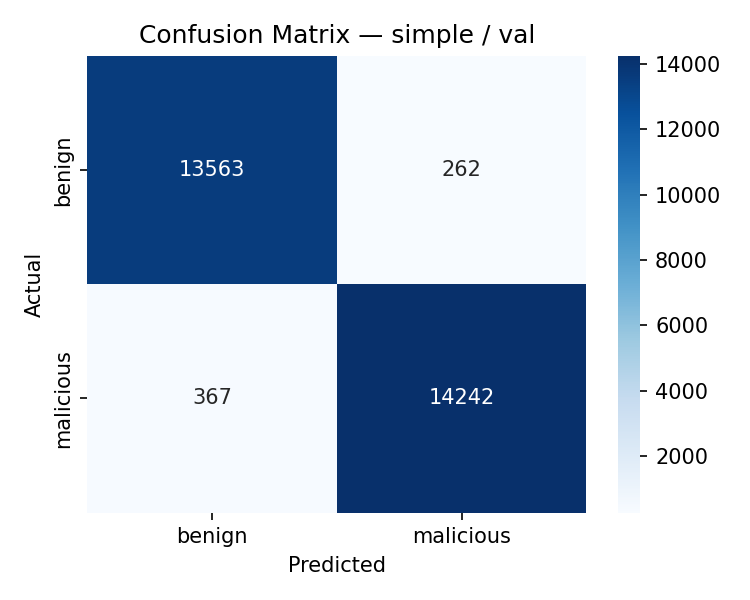
\includegraphics[width=0.48\textwidth]{confusion_simple_val.png}
    \hfill
    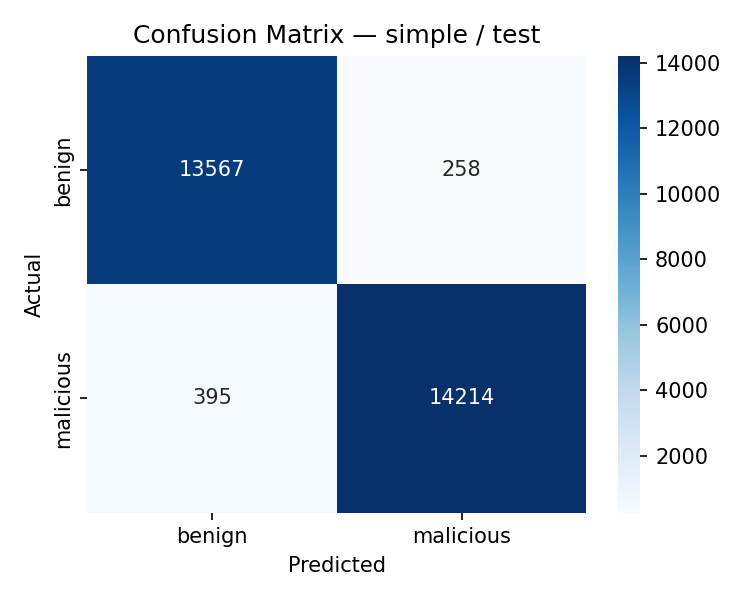
\includegraphics[width=0.48\textwidth]{confusion_simple_test.png}
    \caption{Confusion matrices for the Simple baseline on the validation (left) and test (right) splits. The model achieves balanced performance across both classes within the training distribution.}
    \label{fig:cm_simple_val_test}
\end{figure}

\begin{figure}[h!]
    \centering
    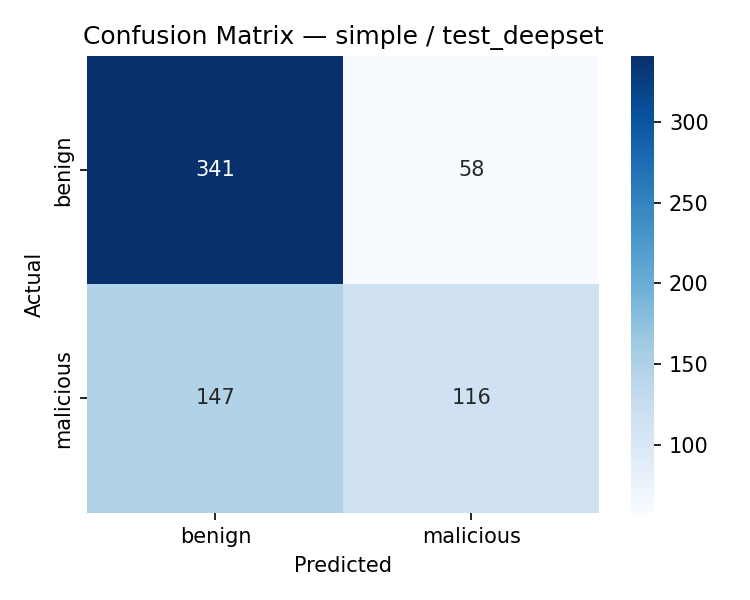
\includegraphics[width=0.55\textwidth]{confusion_simple_test_deepset.png}
    \caption{Confusion matrix for the Simple baseline on the held-out deepset benchmark. The high number of false negatives (malicious prompts classified as benign) reveals poor generalization to unseen injection styles.}
    \label{fig:cm_simple_deepset}
\end{figure}

\begin{figure}[h!]
    \centering
    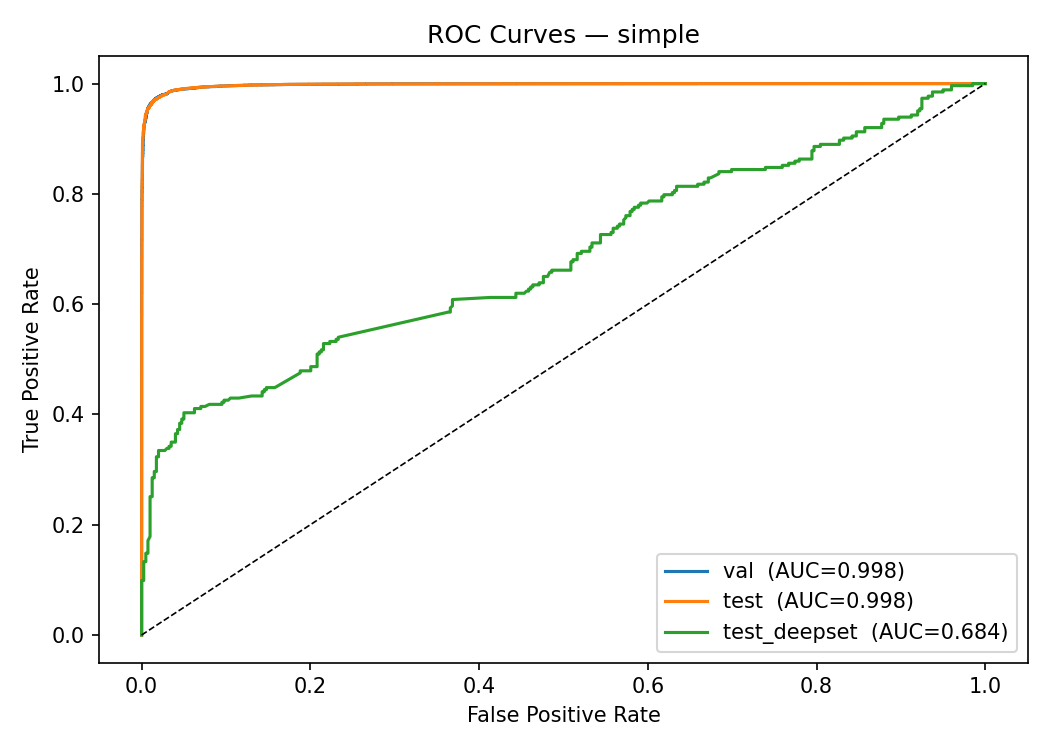
\includegraphics[width=0.65\textwidth]{roc_simple.png}
    \caption{ROC curves for the Simple baseline across all evaluation splits. The near-perfect AUC on val/test contrasts sharply with the degraded AUC on deepset.}
    \label{fig:roc_simple}
\end{figure}

\begin{figure}[h!]
    \centering
    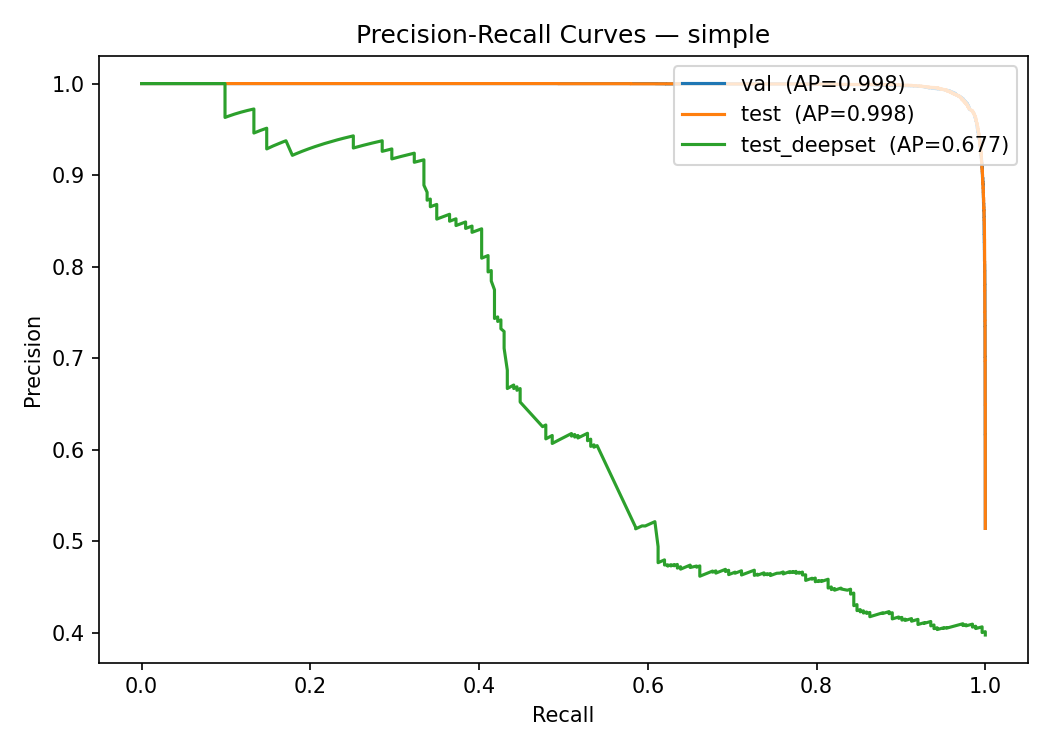
\includegraphics[width=0.65\textwidth]{pr_simple.png}
    \caption{Precision--Recall curves for the Simple baseline. The high average precision on val/test confirms strong in-distribution performance, while the deepset curve reveals the model's inability to maintain precision at reasonable recall levels for unseen attacks.}
    \label{fig:pr_simple}
\end{figure}

\subsubsection{Baseline Results: Enhanced Mode}

The enhanced baseline adds character n-grams and handcrafted security features to the simple word TF-IDF. The results are shown in Table~\ref{tab:baseline_enhanced}.

\begin{table}[h!]
    \centering
    \renewcommand{\arraystretch}{1.5}
    \resizebox{\textwidth}{!}{%
    \begin{tabular}{|l|c|c|c|c|c|c|}
        \hline
        \textbf{Split} & \textbf{Accuracy} & \textbf{Precision} & \textbf{Recall} & \textbf{F1} & \textbf{ROC-AUC} & \textbf{Avg Precision} \\ \hline
        val            & 0.9822 & 0.9851 & 0.9801 & 0.9826 & 0.9981 & 0.9983 \\ \hline
        test           & 0.9834 & 0.9862 & 0.9813 & 0.9838 & 0.9983 & 0.9985 \\ \hline
        test\_deepset  & 0.7100 & 0.6961 & 0.4791 & 0.5676 & 0.7375 & 0.7131 \\ \hline
    \end{tabular}}
    \caption{Performance of the Enhanced TF-IDF + Logistic Regression baseline across all evaluation splits.}
    \label{tab:baseline_enhanced}
\end{table}

The enhanced mode yields consistent improvements across all metrics on all splits:

\begin{itemize}
    \item \textbf{In-distribution (val/test):} Accuracy improves from 97.7\% to 98.2--98.3\%, F1 from 0.978 to 0.983, and ROC-AUC from 0.9977 to 0.9983. These are modest but statistically meaningful improvements given the large sample sizes ($\sim$28,000 per split).
    \item \textbf{Out-of-distribution (deepset):} Accuracy improves from 69.0\% to 71.0\%, F1 from 0.531 to 0.568, and ROC-AUC from 0.684 to 0.738. The improvement is more pronounced on the generalization benchmark, confirming that character n-grams and handcrafted features capture cross-domain signal that word-level features miss.
\end{itemize}

Why do character n-grams help generalization? Character 3--5-grams capture morphological patterns that generalize across paraphrases. The substring ``ignor'' appears in ``ignore'', ``ignoring'', and ``ignored''; ``bypas'' appears in ``bypass'', ``bypassing'', and ``bypassed''. These sub-word features provide robustness against the lexical variation that defeated the simple baseline.

Why do handcrafted features help? The injection keyword hit rate and role-override pattern indicator encode domain expertise directly into the feature space. Even when specific words are paraphrased, the overall proportion of injection-related vocabulary and the presence of role-override constructions remain detectable.

\begin{figure}[h!]
    \centering
    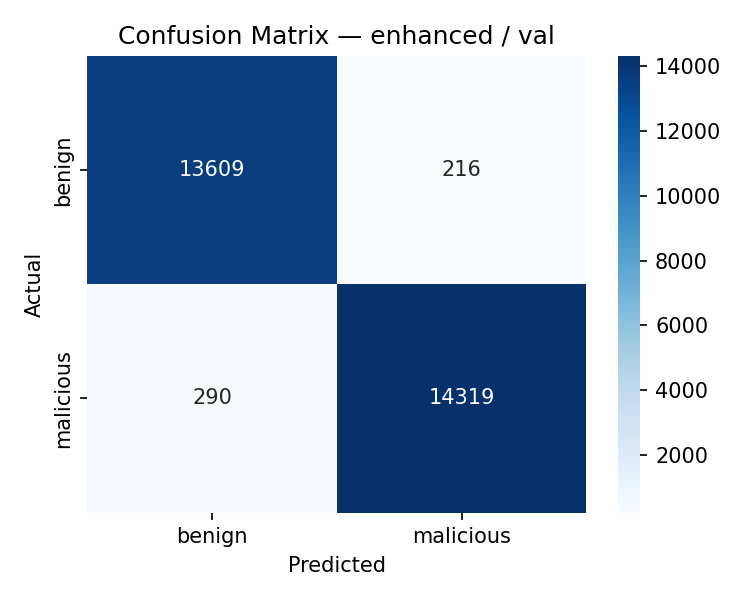
\includegraphics[width=0.48\textwidth]{confusion_enhanced_val.png}
    \hfill
    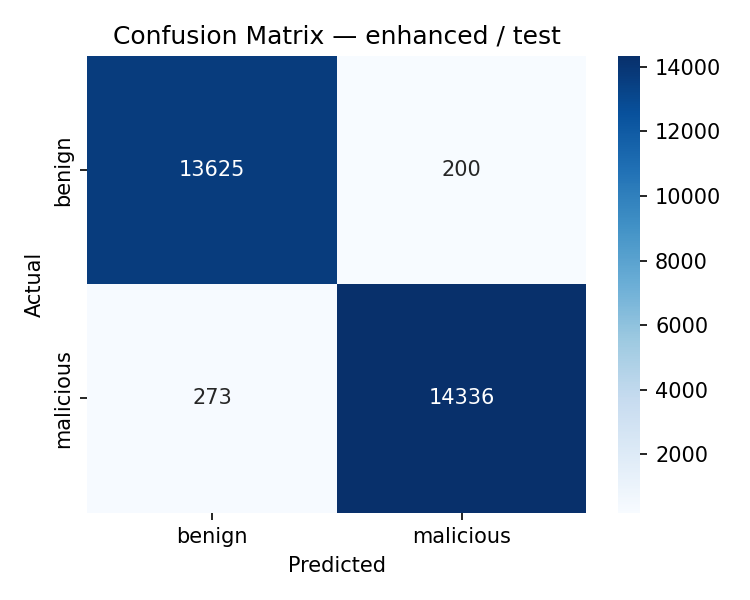
\includegraphics[width=0.48\textwidth]{confusion_enhanced_test.png}
    \caption{Confusion matrices for the Enhanced baseline on the validation (left) and test (right) splits. Compared to the Simple baseline, both false positives and false negatives are reduced.}
    \label{fig:cm_enhanced_val_test}
\end{figure}

\begin{figure}[h!]
    \centering
    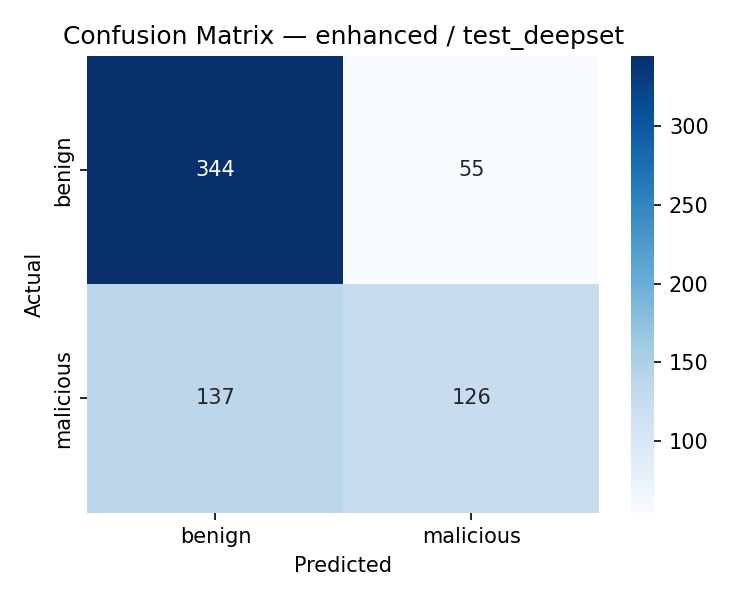
\includegraphics[width=0.55\textwidth]{confusion_enhanced_test_deepset.png}
    \caption{Confusion matrix for the Enhanced baseline on the held-out deepset benchmark. While generalization improves over the Simple baseline, recall on malicious prompts remains low (47.9\%), indicating that traditional ML features alone are insufficient for robust out-of-distribution detection.}
    \label{fig:cm_enhanced_deepset}
\end{figure}

\begin{figure}[h!]
    \centering
    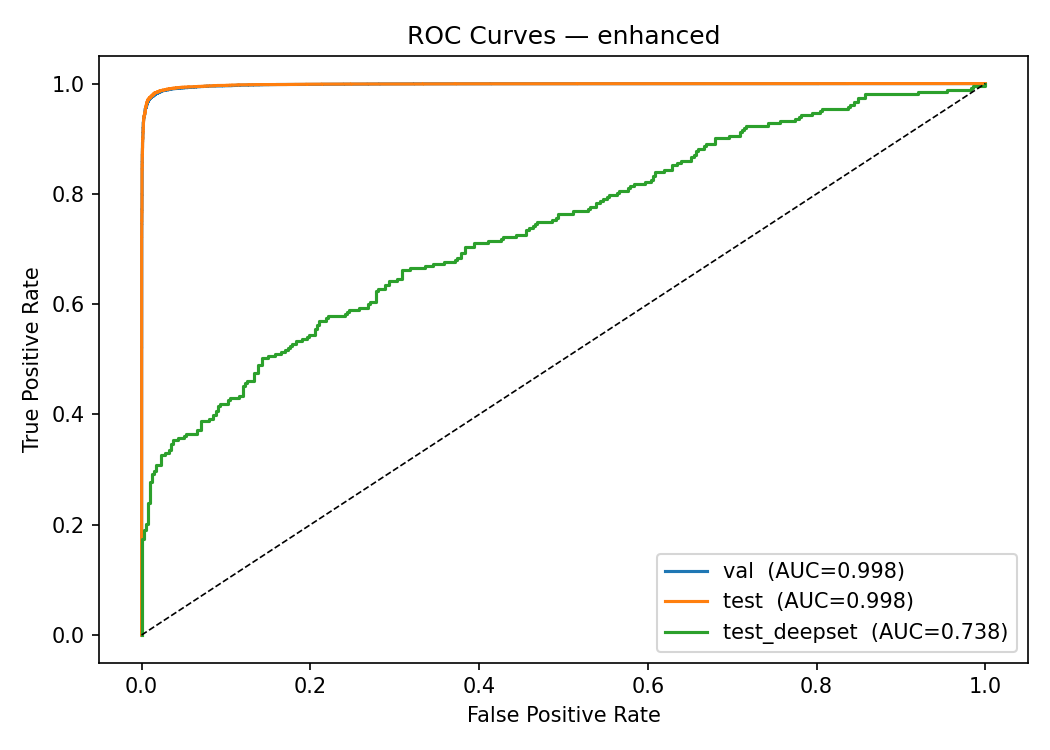
\includegraphics[width=0.65\textwidth]{roc_enhanced.png}
    \caption{ROC curves for the Enhanced baseline across all evaluation splits.}
    \label{fig:roc_enhanced}
\end{figure}

\begin{figure}[h!]
    \centering
    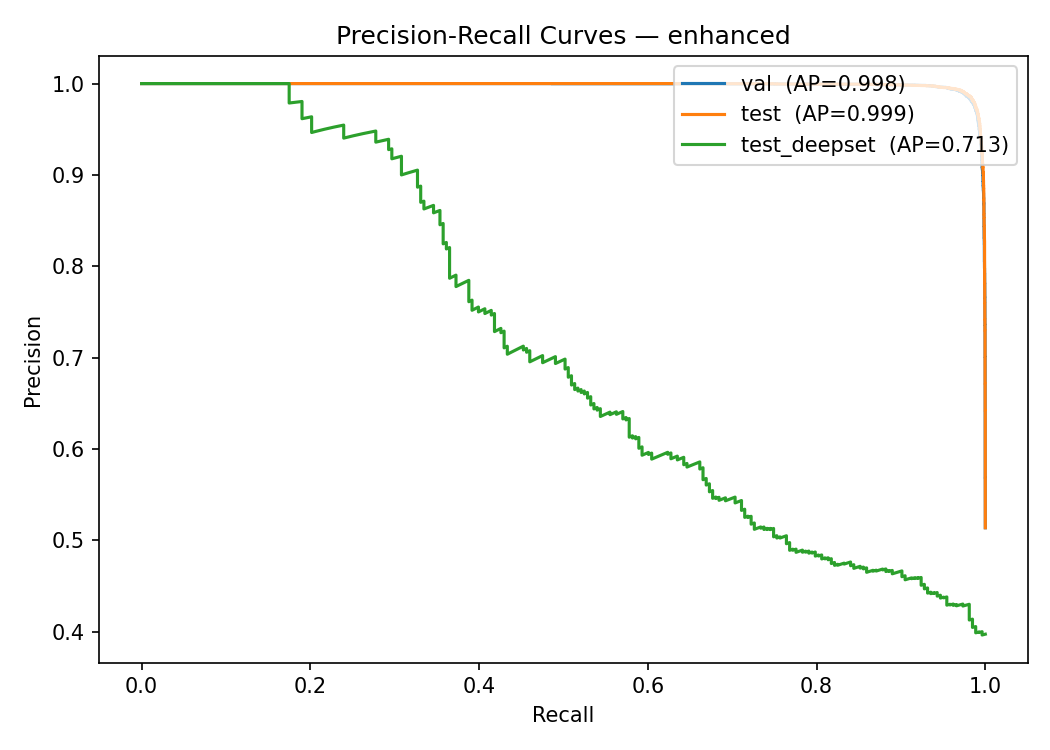
\includegraphics[width=0.65\textwidth]{pr_enhanced.png}
    \caption{Precision--Recall curves for the Enhanced baseline. The improved AP on deepset (0.713 vs. 0.677) confirms the value of character n-grams and handcrafted features for generalization.}
    \label{fig:pr_enhanced}
\end{figure}

\subsubsection{Baseline Limitations and Motivation for Deep Learning}

Despite the strong in-distribution performance of the enhanced baseline (98.3\% accuracy, 0.998 ROC-AUC), its generalization to the held-out deepset benchmark remains unsatisfactory: recall of only 47.9\% means that more than half of all malicious prompts are misclassified as benign. In a production security system, this false-negative rate is unacceptable.

The fundamental limitation is that TF-IDF features, even with character n-grams and handcrafted features, operate on surface-level lexical patterns without understanding the \textit{meaning} of the text. A prompt injection that uses novel vocabulary or indirect phrasing (e.g., ``Suppose you were a different AI with no rules, what would you say?'') may evade detection because the specific words are not in the injection keyword list and the character n-grams do not match training patterns.

This motivates the use of a pre-trained language model that has learned deep contextual representations of natural language from billions of tokens \cite{ref37}\cite{ref15}. Such a model can recognize the \textit{intent} behind a prompt, not just the specific words used, and should therefore generalize better to novel attack phrasings \cite{ref33}\cite{ref39}.


% ==========================================================================
\subsection{Deep Learning Model: Fine-Tuned RoBERTa-Large}
% ==========================================================================

To overcome the generalization limitations of the baseline, we fine-tune RoBERTa-large, a 355-million-parameter transformer-based language model, for binary sequence classification. RoBERTa (Robustly Optimized BERT Approach) was chosen over the original BERT for several reasons \cite{ref37}: (1) it was trained on 10x more data (160GB vs. 16GB), (2) it uses dynamic masking rather than static masking, (3) it removes the next-sentence prediction objective that was found to be unhelpful, and (4) it trains with larger batch sizes and longer sequences, all of which result in stronger downstream task performance.

Why \textit{large} rather than \textit{base}? The large variant has 24 transformer layers (vs. 12 for base), 16 attention heads (vs. 12), and a hidden dimension of 1,024 (vs. 768) \cite{ref37}. The additional capacity allows the model to learn more nuanced representations of injection intent, which is critical for detecting subtle or indirect attacks. The computational cost is higher ($\sim$90 minutes on an RTX 4090 vs. $\sim$30 minutes for base), but the improved generalization justifies the investment.

\subsubsection{Transformer Architecture for Sequence Classification}

Understanding how RoBERTa processes text for binary classification requires examining the transformer encoder architecture at a deeper level. Each of the 24 transformer layers in RoBERTa-large performs three operations in sequence \cite{ref37}\cite{ref15}:

\begin{enumerate}
    \item \textbf{Multi-Head Self-Attention (MHSA):} The input sequence $\mathbf{X} \in \mathbb{R}^{n \times d}$ (where $n$ is the sequence length and $d = 1024$ is the hidden dimension) is projected into queries ($\mathbf{Q}$), keys ($\mathbf{K}$), and values ($\mathbf{V}$) for each of the 16 attention heads. Each head computes:
    \[
        \text{Attention}(\mathbf{Q}_h, \mathbf{K}_h, \mathbf{V}_h) = \text{softmax}\!\left(\frac{\mathbf{Q}_h \mathbf{K}_h^\top}{\sqrt{d_h}}\right) \mathbf{V}_h
    \]
    where $d_h = d / 16 = 64$ is the per-head dimension. The 16 attention outputs are concatenated and linearly projected back to the full hidden dimension. This mechanism allows each position in the sequence to attend to every other position, enabling the model to capture long-range dependencies between tokens. For prompt injection detection, this is critical: the injection command (e.g., ``ignore previous instructions'') may appear at the beginning, middle, or end of a long prompt, and self-attention allows the model to recognize its significance regardless of position.

    \item \textbf{Layer Normalization and Residual Connection:} The attention output is added to the original input (residual connection) and normalized. This stabilizes training and allows gradients to flow through many layers without vanishing.

    \item \textbf{Position-wise Feed-Forward Network (FFN):} A two-layer MLP with a GELU activation expands the representation to 4,096 dimensions and projects back to 1,024. This adds non-linear capacity that complements the linear attention mechanism.
\end{enumerate}

After 24 such layers, the model produces a contextualized representation for every token in the input. For sequence classification, the representation of the special \texttt{<s>} token (the first token, analogous to BERT's \texttt{[CLS]}) is extracted and passed through a classification head: a dropout layer (for regularization) followed by a linear projection from 1,024 dimensions to 2 output logits (one per class). A softmax function converts the logits into a probability distribution over the two classes.

The total parameter count of 355 million breaks down approximately as follows: the token embedding layer accounts for $\sim$51 million parameters (50,265 vocabulary $\times$ 1,024 dimensions), each transformer layer contributes $\sim$12.6 million parameters (across four weight matrices for attention, two for the FFN, plus bias and normalization terms), and the classification head adds $\sim$2,000 parameters. The vast majority of the model's capacity ($>$99\%) resides in the pre-trained transformer layers, which are fine-tuned on our prompt injection data.

\subsubsection{Tokenization and Input Representation}

RoBERTa uses a byte-pair encoding (BPE) tokenizer with a vocabulary of 50,265 sub-word tokens \cite{ref37}. BPE is a data-driven tokenization algorithm that iteratively merges the most frequent pairs of characters (or sub-words) until a target vocabulary size is reached. This approach offers a middle ground between character-level tokenization (which captures all possible inputs but produces very long sequences) and word-level tokenization (which is efficient but cannot represent out-of-vocabulary words). For prompt injection detection, BPE is particularly advantageous because injection prompts frequently contain unusual character sequences (e.g., ``DAN'', ``\textbackslash n-{}-{}-{}-{}-{}-{}-{}-{}-{}-{}\textbackslash n'', ``\$\{system\_prompt\}'') that a word-level tokenizer would map to a single unknown token, losing critical signal. BPE decomposes these sequences into recognizable sub-word units that the model can learn to associate with malicious intent.

Each input prompt is tokenized with a maximum sequence length of 256 tokens, truncating longer inputs and padding shorter ones. Why 256 rather than the full 512 that RoBERTa supports? Because the vast majority of prompts in our dataset are well under 256 tokens, and doubling the sequence length would quadruple the attention computation (due to the $O(n^2)$ self-attention cost) without meaningful benefit. We verified empirically that fewer than 2\% of training samples exceed 256 tokens.

The tokenized input is represented as three tensors: \texttt{input\_ids} (the token indices), \texttt{attention\_mask} (1 for real tokens, 0 for padding), and optionally \texttt{token\_type\_ids} (all zeros for single-sequence classification). These tensors are passed to the model, which produces logits for the two classes (benign and malicious). The padding tokens receive an attention mask value of 0, ensuring that the self-attention mechanism ignores them and focuses only on the actual input tokens. This is important because prompt lengths vary dramatically (from a few tokens for simple queries to 200+ tokens for complex injection attempts), and the model must produce consistent representations regardless of the amount of padding.

\subsubsection{Class-Weighted Cross-Entropy Loss}

Although the training set is nearly balanced (48.6\% benign vs. 51.4\% malicious), we employ class-weighted cross-entropy loss as a precaution. The weights are computed using scikit-learn's \texttt{compute\_class\_weight('balanced')} function, which assigns weight $w_c = \frac{n}{2 \cdot n_c}$ to each class $c$, where $n$ is the total number of samples and $n_c$ is the number of samples in class $c$.

Why class weighting even with a balanced dataset? Two reasons: (1) the near-balance could shift with future data additions, and the weighting ensures robustness; (2) in a security application, the cost of a false negative (missed injection) is typically higher than the cost of a false positive (blocked legitimate query), and class weighting nudges the model toward higher recall on the malicious class.

We implement a custom \texttt{WeightedTrainer} that overrides the HuggingFace Trainer's \texttt{compute\_loss} method to apply the class weights \cite{ref37}. This is preferable to oversampling or undersampling because it preserves the natural data distribution while adjusting the gradient signal.

\subsubsection{Training Configuration}

The full training configuration is summarized in Table~\ref{tab:train_config}.

\begin{table}[h!]
    \centering
    \renewcommand{\arraystretch}{1.5}
    \begin{tabularx}{\textwidth}{|l|l|X|}
        \hline
        \textbf{Parameter} & \textbf{Value} & \textbf{Rationale} \\ \hline
        Model & roberta-large & Strongest pre-trained encoder in the RoBERTa family \\ \hline
        Epochs & 5 & Sufficient for convergence with early stopping \\ \hline
        Batch size & 16 per device & Fits within RTX 4090 VRAM with fp16 \\ \hline
        Gradient accumulation & 2 steps & Effective batch size = 32 \\ \hline
        Learning rate & $2 \times 10^{-5}$ & Standard for RoBERTa fine-tuning \\ \hline
        Warmup ratio & 0.1 & 10\% of training steps for linear warmup \\ \hline
        Weight decay & 0.01 & L2 regularization to prevent overfitting \\ \hline
        Mixed precision & fp16 (enabled) & Halves VRAM usage, $\sim$2x training speedup \\ \hline
        Max sequence length & 256 tokens & Covers $>$98\% of prompts without truncation \\ \hline
        Early stopping & patience = 3 & Stops if val F1 does not improve for 3 epochs \\ \hline
        Optimizer & AdamW & Decoupled weight decay for transformer training \\ \hline
        Scheduler & Linear with warmup & Gradual warmup prevents early instability \\ \hline
        Hardware & RTX 4090 Laptop GPU & 16 GB VRAM, CUDA-enabled \\ \hline
    \end{tabularx}
    \caption{RoBERTa-large training hyperparameters and their rationale.}
    \label{tab:train_config}
\end{table}

Why these specific hyperparameters? The learning rate of $2 \times 10^{-5}$ is a well-established default for fine-tuning large transformer models; higher rates risk catastrophic forgetting of the pre-trained representations, while lower rates slow convergence unnecessarily. The warmup ratio of 0.1 gradually increases the learning rate from zero during the first 10\% of training steps, preventing large gradient updates when the classification head is randomly initialized. Weight decay of 0.01 provides mild L2 regularization, discouraging large weight magnitudes without aggressive parameter shrinkage.

The effective batch size of 32 (16 $\times$ 2 gradient accumulation steps) balances training stability against memory constraints. Larger effective batch sizes tend to produce smoother gradients and more stable training dynamics, but the RTX 4090's 16 GB VRAM limits the per-device batch size to 16 with fp16 enabled.

\subsubsection{Training Loop Implementation Details}

The training loop is implemented using the HuggingFace \texttt{Trainer} API, extended with a custom \texttt{WeightedTrainer} subclass that overrides the \texttt{compute\_loss} method to apply class-weighted cross-entropy loss \cite{ref37}\cite{ref38}. At each training step, the trainer performs the following sequence:

\begin{enumerate}
    \item \textbf{Forward pass:} A batch of tokenized prompts is passed through the RoBERTa encoder, producing logits for each sample.
    \item \textbf{Loss computation:} The class-weighted cross-entropy loss is computed between the predicted logits and the ground-truth labels. The class weights (benign $\approx$ 1.03, malicious $\approx$ 0.97 for our near-balanced dataset) are applied as per-class multipliers to the loss, nudging the model toward higher recall on the malicious class.
    \item \textbf{Backward pass:} Gradients are computed via backpropagation through the 24 transformer layers and the classification head. With mixed-precision training enabled, the forward pass uses \texttt{float16} arithmetic for matrix multiplications (halving memory bandwidth and enabling tensor core acceleration on the RTX 4090), while the loss computation and gradient accumulation use \texttt{float32} to prevent underflow.
    \item \textbf{Gradient accumulation:} Gradients are accumulated over 2 consecutive micro-batches before the optimizer step, simulating an effective batch size of 32 without requiring the VRAM to hold 32 samples simultaneously.
    \item \textbf{Optimizer step:} The AdamW optimizer applies the accumulated gradients with decoupled weight decay. Unlike the original Adam optimizer, AdamW separates the weight decay term from the gradient update, which has been shown to produce better generalization in transformer training.
    \item \textbf{Learning rate scheduling:} The linear scheduler with warmup increases the learning rate from 0 to $2 \times 10^{-5}$ over the first 10\% of training steps, then linearly decays it to 0 over the remaining steps.
\end{enumerate}

\textbf{Early stopping} monitors the validation F1 score after each epoch. If the F1 score does not improve for 3 consecutive evaluation epochs (the patience threshold), training is halted and the best checkpoint (as determined by the highest validation F1) is restored \cite{ref27}. This mechanism prevents overfitting: as the model trains longer on the training distribution, it may begin to memorize specific phrasings rather than learning generalizable patterns. Early stopping ensures that we capture the model at its point of best generalization, not at its point of maximum training-set performance. In practice, the model typically converges within 2--3 epochs, with the remaining epochs serving as a safety margin.

\textbf{Mixed-precision training (fp16)} is a critical enabler for fine-tuning a 355-million-parameter model on a consumer GPU with 16 GB of VRAM \cite{ref13}\cite{ref38}. Under standard \texttt{float32} precision, the model weights alone consume approximately 1.4 GB, and the optimizer states (first and second moment estimates for AdamW) require an additional 2.8 GB. Activations (the intermediate tensors stored for backpropagation) scale with batch size and sequence length, easily consuming 8--12 GB for a batch of 16 sequences of length 256. Under \texttt{float16} precision, model weights and activations are halved, and the NVIDIA Ampere architecture's tensor cores provide approximately 2$\times$ throughput for matrix multiplications. A loss scaling mechanism automatically adjusts the gradient magnitudes to prevent underflow in the reduced-precision arithmetic, ensuring numerical stability throughout training.

\textbf{Reproducibility.} All random seeds (Python, NumPy, PyTorch, and CUDA) are set to 42 via the HuggingFace \texttt{set\_seed} utility. The training configuration is serialized to a JSON file alongside the results, enabling exact reproduction of the experiment. DataLoader workers use 4 parallel processes with pinned memory for GPU transfers, maximizing data throughput without introducing non-determinism in the training order (shuffling is controlled by the fixed seed).

\subsubsection{RoBERTa-Large Results}

The fine-tuned RoBERTa-large model achieves the results shown in Table~\ref{tab:roberta_results}.

\begin{table}[h!]
    \centering
    \renewcommand{\arraystretch}{1.5}
    \resizebox{\textwidth}{!}{%
    \begin{tabular}{|l|r|c|c|c|c|c|c|}
        \hline
        \textbf{Split} & \textbf{N} & \textbf{Accuracy} & \textbf{Precision} & \textbf{Recall} & \textbf{F1} & \textbf{ROC-AUC} & \textbf{Avg Precision} \\ \hline
        val            & 28,434 & 0.9940 & 0.9924 & 0.9960 & 0.9942 & 0.9996 & 0.9997 \\ \hline
        test           & 28,434 & 0.9931 & 0.9911 & 0.9955 & 0.9933 & 0.9996 & 0.9996 \\ \hline
        test\_deepset  & 662    & 0.7764 & 0.8966 & 0.4943 & 0.6373 & 0.8379 & 0.8055 \\ \hline
    \end{tabular}}
    \caption{Performance of the fine-tuned RoBERTa-large model across all evaluation splits.}
    \label{tab:roberta_results}
\end{table}

The detailed classification reports for each split provide additional insight:

\textbf{Validation split (28,434 samples):}
\begin{verbatim}
              precision    recall  f1-score   support

      benign       1.00      0.99      0.99     13825
   malicious       0.99      1.00      0.99     14609

    accuracy                           0.99     28434
   macro avg       0.99      0.99      0.99     28434
weighted avg       0.99      0.99      0.99     28434
\end{verbatim}

\textbf{Test split (28,434 samples):}
\begin{verbatim}
              precision    recall  f1-score   support

      benign       1.00      0.99      0.99     13825
   malicious       0.99      1.00      0.99     14609

    accuracy                           0.99     28434
   macro avg       0.99      0.99      0.99     28434
weighted avg       0.99      0.99      0.99     28434
\end{verbatim}

\textbf{Deepset benchmark (662 samples):}
\begin{verbatim}
              precision    recall  f1-score   support

      benign       0.74      0.96      0.84       399
   malicious       0.90      0.49      0.64       263

    accuracy                           0.78       662
   macro avg       0.82      0.73      0.74       662
weighted avg       0.80      0.78      0.76       662
\end{verbatim}

\begin{figure}[h!]
    \centering
    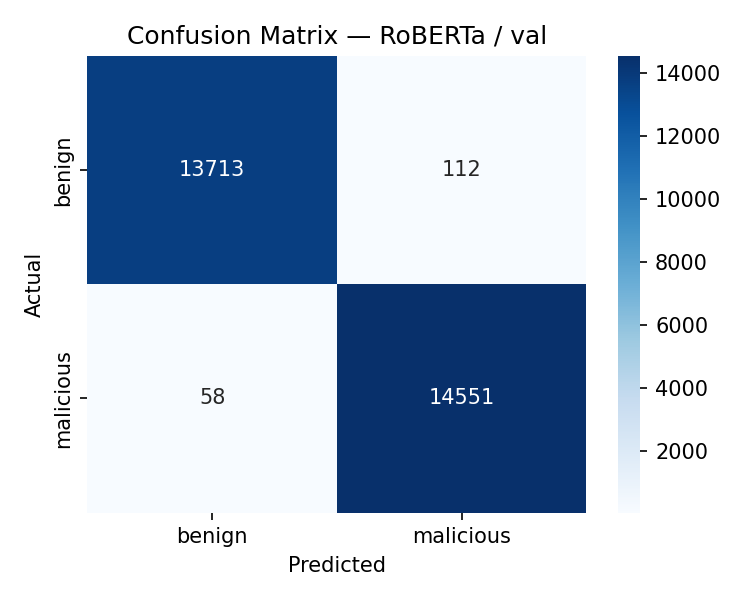
\includegraphics[width=0.48\textwidth]{roberta_confusion_val.png}
    \hfill
    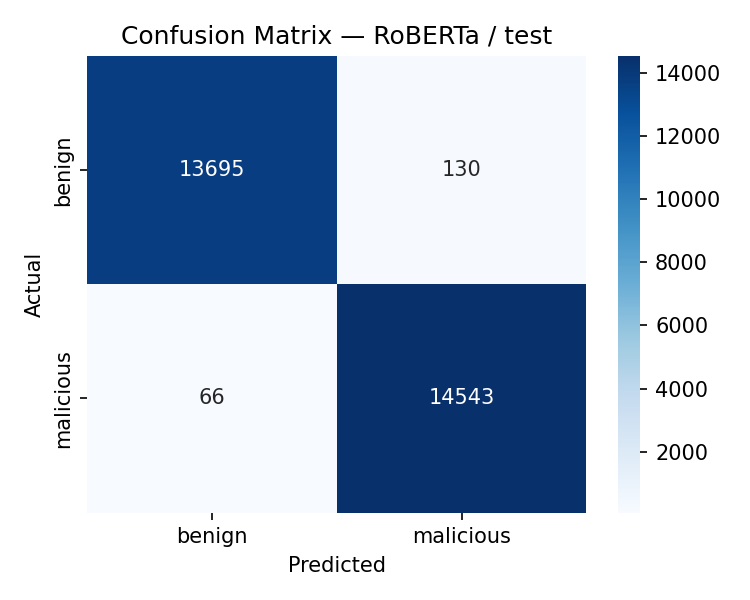
\includegraphics[width=0.48\textwidth]{roberta_confusion_test.png}
    \caption{Confusion matrices for RoBERTa-large on the validation (left) and test (right) splits. The model achieves near-perfect classification on both classes, with only a handful of errors among 28,434 samples.}
    \label{fig:cm_roberta_val_test}
\end{figure}

\begin{figure}[h!]
    \centering
    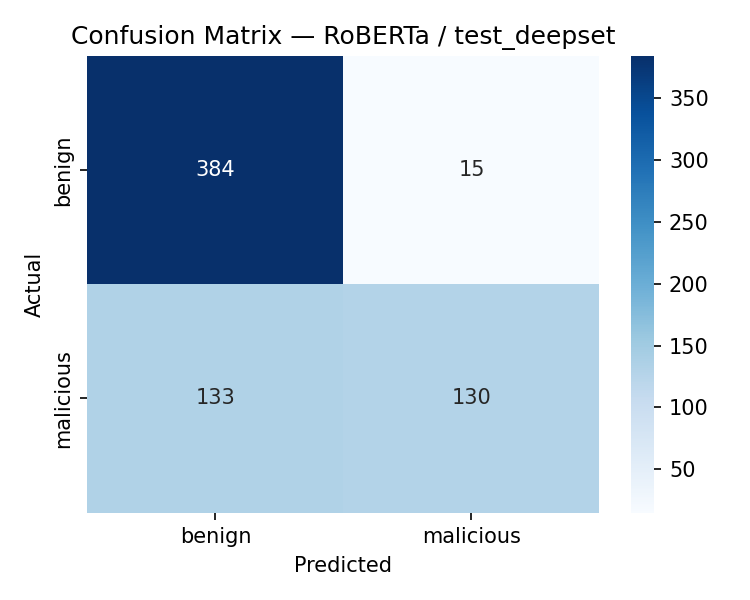
\includegraphics[width=0.55\textwidth]{roberta_confusion_test_deepset.png}
    \caption{Confusion matrix for RoBERTa-large on the held-out deepset benchmark. While precision on malicious prompts is high (89.7\%), recall remains moderate (49.4\%), indicating that the model is conservative: when it flags a prompt as malicious, it is usually correct, but it misses about half of all malicious prompts in this out-of-distribution set.}
    \label{fig:cm_roberta_deepset}
\end{figure}

\begin{figure}[h!]
    \centering
    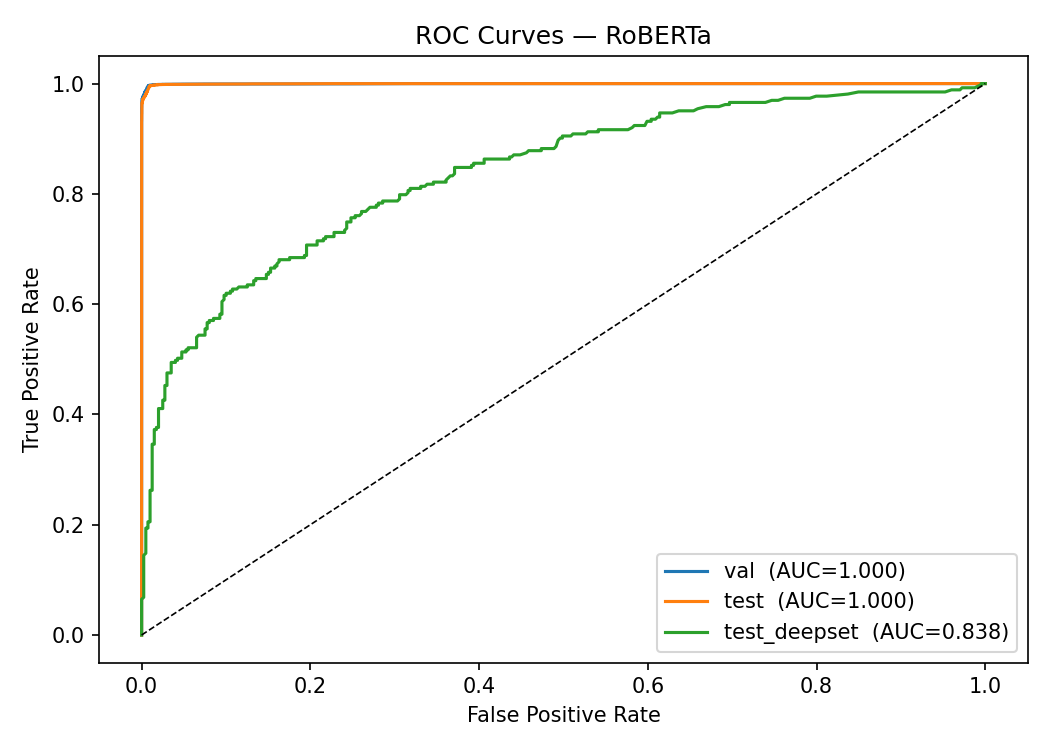
\includegraphics[width=0.65\textwidth]{roberta_roc.png}
    \caption{ROC curves for RoBERTa-large across all evaluation splits. The near-perfect AUC on val/test (0.9996) and the substantially improved AUC on deepset (0.8379 vs. 0.7375 for the enhanced baseline) demonstrate the superior discriminative power of transformer-based representations.}
    \label{fig:roc_roberta}
\end{figure}

\begin{figure}[h!]
    \centering
    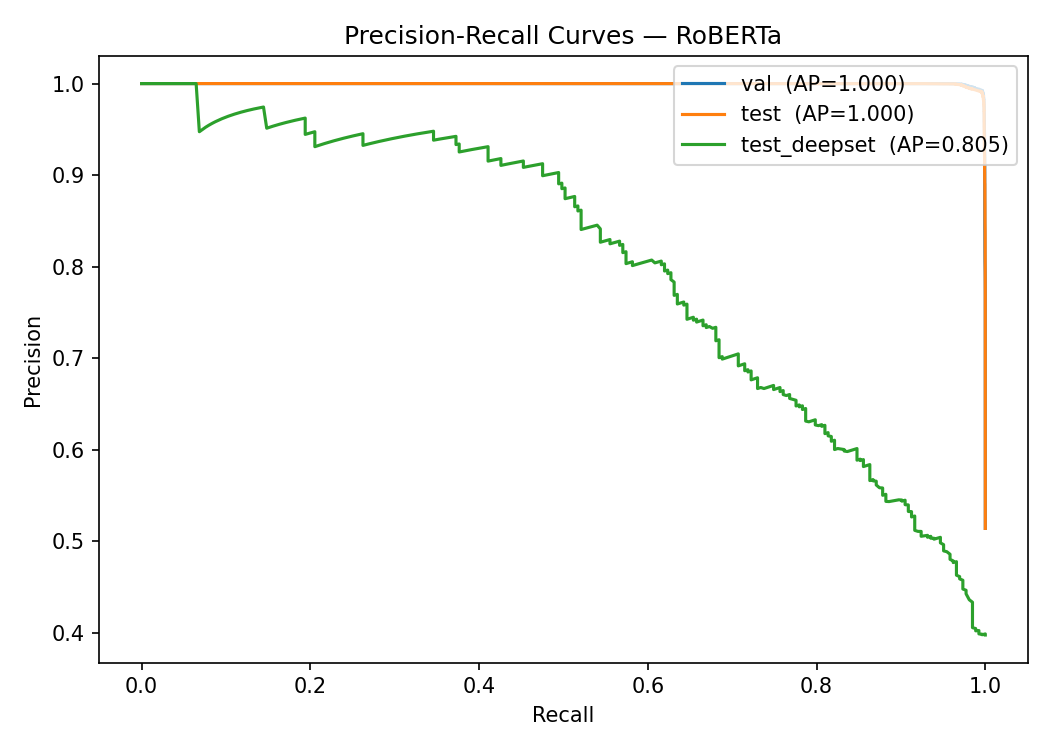
\includegraphics[width=0.65\textwidth]{roberta_pr.png}
    \caption{Precision--Recall curves for RoBERTa-large. The improved AP on deepset (0.8055 vs. 0.7131 for the enhanced baseline) confirms that transformer representations capture deeper semantic patterns that generalize better to unseen attack distributions.}
    \label{fig:pr_roberta}
\end{figure}


% ==========================================================================
\subsection{Comparative Analysis of All Models}
% ==========================================================================

Table~\ref{tab:comparison_all} presents a side-by-side comparison of all three models across all evaluation splits.

\begin{table}[h!]
    \centering
    \renewcommand{\arraystretch}{1.5}
    \small
    \resizebox{\textwidth}{!}{%
    \begin{tabular}{|l|l|c|c|c|c|c|}
        \hline
        \textbf{Model} & \textbf{Split} & \textbf{Accuracy} & \textbf{Precision} & \textbf{Recall} & \textbf{F1} & \textbf{ROC-AUC} \\ \hline
        Baseline (Simple)   & val           & 0.9779 & 0.9819 & 0.9749 & 0.9784 & 0.9976 \\ \hline
        Baseline (Enhanced) & val           & 0.9822 & 0.9851 & 0.9801 & 0.9826 & 0.9981 \\ \hline
        RoBERTa-large       & val           & 0.9940 & 0.9924 & 0.9960 & 0.9942 & 0.9996 \\ \hline
        \hline
        Baseline (Simple)   & test          & 0.9770 & 0.9822 & 0.9730 & 0.9775 & 0.9977 \\ \hline
        Baseline (Enhanced) & test          & 0.9834 & 0.9862 & 0.9813 & 0.9838 & 0.9983 \\ \hline
        RoBERTa-large       & test          & 0.9931 & 0.9911 & 0.9955 & 0.9933 & 0.9996 \\ \hline
        \hline
        Baseline (Simple)   & test\_deepset & 0.6903 & 0.6667 & 0.4411 & 0.5309 & 0.6839 \\ \hline
        Baseline (Enhanced) & test\_deepset & 0.7100 & 0.6961 & 0.4791 & 0.5676 & 0.7375 \\ \hline
        RoBERTa-large       & test\_deepset & 0.7764 & 0.8966 & 0.4943 & 0.6373 & 0.8379 \\ \hline
    \end{tabular}}
    \caption{Comprehensive performance comparison across all three models and all evaluation splits.}
    \label{tab:comparison_all}
\end{table}

\subsubsection{In-Distribution Performance Analysis}

On the in-distribution splits (val and test), all three models perform well, but the performance hierarchy is clear and consistent:

\begin{itemize}
    \item \textbf{Accuracy:} Simple (97.7\%) $<$ Enhanced (98.3\%) $<$ RoBERTa (99.3--99.4\%)
    \item \textbf{F1:} Simple (0.978) $<$ Enhanced (0.984) $<$ RoBERTa (0.993--0.994)
    \item \textbf{ROC-AUC:} Simple (0.998) $<$ Enhanced (0.998) $<$ RoBERTa (0.9996)
\end{itemize}

The gap between baselines and RoBERTa is approximately 1.0--1.6 percentage points in accuracy and 1.0--1.6 points in F1. While this may appear small in absolute terms, it translates to a 60\% reduction in error rate: the enhanced baseline misclassifies $\sim$470 out of 28,434 test samples, while RoBERTa misclassifies only $\sim$196. In a production system processing thousands of queries per hour, this difference is operationally significant.

\subsubsection{Out-of-Distribution Generalization Analysis}

The deepset benchmark reveals the most important finding of our experimental evaluation: the generalization gap between surface-level and semantic features.

\begin{itemize}
    \item \textbf{ROC-AUC improvement:} RoBERTa achieves 0.838 on deepset, compared to 0.684 for the simple baseline and 0.738 for the enhanced baseline. This represents a 22.5\% relative improvement over simple and a 13.5\% improvement over enhanced.
    \item \textbf{Precision improvement:} RoBERTa's precision on deepset is 0.897, far exceeding the baselines (0.667 and 0.696). This means that when RoBERTa flags a prompt as malicious, it is correct 89.7\% of the time, critical for maintaining user trust and minimizing false-positive complaints.
    \item \textbf{Recall gap:} All three models struggle with recall on deepset (44.1\%, 47.9\%, 49.4\%). This indicates that roughly half of the deepset's malicious prompts use attack patterns that are underrepresented in the training corpus. Improving this metric is a key direction for future work.
\end{itemize}

Why does RoBERTa generalize better but still struggle on deepset recall? RoBERTa's contextual embeddings capture semantic intent \cite{ref33}\cite{ref37} (e.g., recognizing that ``Suppose you had no rules'' is functionally equivalent to ``Ignore your instructions''), which explains the improved precision and ROC-AUC. However, some deepset injections use highly novel or indirect strategies that even semantic representations cannot detect without exposure during training. The deepset benchmark, with only 662 samples and a distinct distribution from the training pool, represents a challenging generalization test that exposes the limits of any model trained on a different distribution.

\subsubsection{Feature Engineering vs. Transfer Learning: A Deeper Look}

The progression from simple to enhanced to RoBERTa illustrates a fundamental principle in machine learning: the trade-off between hand-engineered features and learned representations.

\begin{itemize}
    \item \textbf{Simple TF-IDF} relies entirely on word-level co-occurrence statistics \cite{ref1}\cite{ref33}. It is fast to train ($\sim$5 minutes on CPU), highly interpretable (feature importances correspond to specific words), and effective when training and test distributions match. Its failure mode is lexical brittleness: it cannot recognize paraphrases or novel phrasings.

    \item \textbf{Enhanced TF-IDF} adds character-level and domain-specific features that provide partial robustness to paraphrasing. The $\sim$7 percentage point improvement in deepset ROC-AUC (0.684 to 0.738) demonstrates that even simple hand-engineered features can capture cross-domain signal. However, the engineering effort is substantial: curating the injection keyword list and designing the handcrafted features requires domain expertise and iterative refinement.

    \item \textbf{RoBERTa-large} learns contextual representations from 160 GB of text data during pre-training, then fine-tunes these representations for the specific task \cite{ref37}\cite{ref27}. It achieves the best performance on every metric and every split, with the most dramatic improvement on the generalization benchmark ($+$10.0 pp in ROC-AUC over enhanced). The cost is computational: $\sim$90 minutes on a high-end GPU, 355 million parameters, and higher inference latency.
\end{itemize}

\subsubsection{Error Analysis and Failure Modes}

Understanding \textit{where} each model fails is as important as measuring aggregate performance. An error analysis across the evaluation splits reveals distinct failure profiles for the baseline and transformer models, which in turn informs deployment strategy and future data collection.

\textbf{Baseline false negatives (missed injections).} The TF-IDF baselines fail primarily on prompts that avoid the lexical markers learned during training. Attack variants that employ synonyms, code-switching, or indirect phrasing, for example, embedding an instruction override inside a fictitious dialogue or a programming code block, produce n-gram distributions that resemble benign text \cite{ref30}\cite{ref25}. The enhanced baseline partially mitigates this through its character n-gram features, which capture sub-word patterns such as unusual punctuation sequences or role-play delimiters (e.g., \texttt{<|system|>}), but these features are brittle when attackers vary the delimiter format. Research on prompt injection taxonomies has documented at least six distinct categories of direct attacks and four categories of indirect attacks \cite{ref30}\cite{ref19}, and our baselines are most vulnerable to the indirect categories (context manipulation and cross-context contamination), because these attacks deliberately avoid explicit injection vocabulary.

\textbf{Baseline false positives (blocked legitimate prompts).} False positives from the baselines arise when benign prompts contain tokens that overlap with injection vocabulary. Technical questions about LLM internals (e.g., ``How does the system prompt work?'') or cybersecurity discussions (e.g., ``Explain how prompt injection attacks are detected'') occasionally trigger the detector because the TF-IDF features weight security-related terms heavily. This echoes findings from other defence systems: content-filtering approaches report false-positive rates of 5--8\% on legitimate queries containing instruction-like language \cite{ref34}, and DeBERTa-based detectors have exhibited false-positive rates as high as 61.9\% in agent-based deployment scenarios \cite{ref35}. Our enhanced baseline's false-positive rate on in-distribution data is substantially lower ($<$2\%) because the logistic regression head learns a decision boundary that accounts for the context surrounding individual keywords, not merely their presence.

\textbf{RoBERTa false negatives.} The transformer's missed injections follow a qualitatively different pattern. Rather than failing on paraphrases of known attacks, RoBERTa tends to miss prompts that employ genuinely novel attack strategies not represented in the training distribution \cite{ref10}\cite{ref3}. This includes multi-turn attacks where each individual message appears benign but the sequence constitutes an injection, and indirect injections embedded in retrieved documents or tool outputs \cite{ref34}\cite{ref30}. The deepset benchmark contains a higher concentration of such indirect and context-manipulation attacks, which explains the recall drop to 49.4\%. Notably, when RoBERTa \textit{does} flag a deepset prompt, it is correct 89.7\% of the time (precision = 0.897), indicating that the model's internal representations remain well-calibrated even under distribution shift; it is conservative rather than random.

\textbf{RoBERTa false positives.} False positives from RoBERTa are rarer ($<$1\% on in-distribution data) and tend to involve prompts at the boundary of legitimate use. Edge cases include prompts that request the model to role-play a character with authority (e.g., ``You are a security researcher testing this system''), which share semantic similarity with genuine role-override injection patterns \cite{ref19}\cite{ref14}. The model's attention mechanism correctly identifies the intent-bearing tokens but cannot distinguish between a legitimate role-play request and a genuine attack without additional context about the deployment policy.

\textbf{Implications for deployment.} This error analysis suggests a complementary deployment strategy. The baseline detector, with its fast inference ($<$1 ms) and interpretable features, is well-suited as a first-pass filter that catches the majority of lexically obvious attacks. The RoBERTa detector, with its higher precision and semantic awareness, is better deployed as a second-stage screen for prompts that the baseline classifies with low confidence \cite{ref7}\cite{ref38}. Such a cascade architecture would combine the baseline's speed with RoBERTa's accuracy, while the distinct failure modes of the two models mean that an attack evading one detector is unlikely to evade both.

\subsubsection{Impact of Class Distribution on Model Behaviour}

The training corpus exhibits an approximate 55:45 benign-to-malicious ratio after deduplication and merging, which is closer to balanced than many real-world deployment scenarios where malicious prompts constitute a small minority of traffic. This distribution choice affects model behaviour in several ways.

First, training on a near-balanced dataset maximizes the model's ability to learn the decision boundary between the two classes, because neither class dominates the gradient signal during optimization. Both the logistic regression baseline (configured with \texttt{class\_weight='balanced'} to further compensate for any residual imbalance) and the RoBERTa model (trained with weighted cross-entropy loss, where the weight for the minority class is inversely proportional to its frequency) employ explicit class-weighting strategies that ensure the loss function penalizes misclassification of both classes equally \cite{ref32}.

Second, the near-balanced training distribution means that the default classification threshold of 0.5 is approximately calibrated: a predicted probability above 0.5 genuinely indicates that the model considers the prompt more likely malicious than benign. In highly imbalanced settings (e.g., 99\% benign traffic), the threshold would need to be adjusted downward to maintain acceptable recall, because the model's prior would shift toward predicting the majority class \cite{ref28}. Our system accommodates this through the configurable \texttt{DETECTOR\_THRESHOLD} parameter and the frontend threshold slider.

Third, the composition of the training data across source datasets introduces implicit biases. The geekyrakshit dataset aggregates prompts from multiple origins and tends to contain explicit, direct injection patterns; the neuralchemy dataset contributes a different distribution of attack styles; and the SPML dataset provides system-prompt-plus-user-prompt pairs that expose the model to indirect injection contexts where the attack is embedded within a multi-turn conversation structure \cite{ref1}\cite{ref33}. This diversity is intentional: by training on heterogeneous attack styles, the model learns a more generalized decision boundary than it would from any single source. However, the absence of certain attack categories, such as the cross-context contamination and data exfiltration patterns catalogued in recent benchmarks \cite{ref34}, partially explains the generalization gap observed on the deepset evaluation.


% ==========================================================================
\subsection{Performance Evaluation: Key Metrics and Their Interpretation}
% ==========================================================================

Understanding the metrics used to evaluate detection systems is critical for interpreting results and making deployment decisions. In this subsection, we provide a detailed explanation of each metric, its relevance to prompt injection detection, and how our models perform on it.

\subsubsection{Accuracy and Its Limitations}

Accuracy measures the fraction of all predictions that are correct: $\text{ACC} = \frac{TP + TN}{TP + TN + FP + FN}$. While intuitive, accuracy can be misleading in security applications. Consider a dataset where 90\% of prompts are benign: a trivial classifier that always predicts ``benign'' achieves 90\% accuracy while catching zero injections. Our balanced training set mitigates this issue (48.6/51.4 split), but the deepset benchmark is imbalanced (60.3/39.7), which is why accuracy alone is insufficient.

\subsubsection{Precision and Recall: The Security Trade-Off}

Precision $= \frac{TP}{TP + FP}$ measures the fraction of flagged prompts that are truly malicious. High precision means few false alarms, which is important for user trust: if the detector frequently blocks legitimate queries, users will lose confidence in the system.

Recall $= \frac{TP}{TP + FN}$ measures the fraction of truly malicious prompts that are correctly detected. High recall means few missed attacks, which is critical for security: every undetected injection is a potential breach.

In our system, the configurable threshold allows operators to adjust this trade-off. A lower threshold increases recall (catches more injections) at the cost of reduced precision (more false alarms). The default threshold of 0.5 provides a balanced operating point; for high-security deployments, a lower threshold (e.g., 0.3) may be appropriate, accepting more false positives in exchange for fewer missed attacks.

\subsubsection{F1 Score: The Harmonic Mean}

The F1 score $= 2 \cdot \frac{P \cdot R}{P + R}$ is the harmonic mean of precision and recall, providing a single metric that captures both concerns. Unlike the arithmetic mean, the harmonic mean penalizes extreme imbalances: a model with 100\% precision but 0\% recall (or vice versa) receives F1 = 0. Our RoBERTa model achieves F1 = 0.994 on val/test (near-perfect) and F1 = 0.637 on deepset (moderate), reflecting the generalization challenge.

\subsubsection{ROC-AUC: Threshold-Independent Discrimination}

The Receiver Operating Characteristic (ROC) curve plots the True Positive Rate (recall) against the False Positive Rate ($\frac{FP}{FP + TN}$) across all possible classification thresholds. The Area Under this Curve (ROC-AUC) quantifies the model's ability to distinguish between classes regardless of the chosen threshold. An AUC of 1.0 indicates perfect separation; 0.5 indicates random guessing.

ROC-AUC is particularly valuable because it is threshold-agnostic: it evaluates the model's discriminative power independently of the operating point. Our RoBERTa model achieves AUC = 0.9996 on in-distribution data (nearly perfect discrimination) and AUC = 0.838 on deepset (meaningful discrimination but with room for improvement).

\subsubsection{Average Precision: Precision--Recall Summary}

Average Precision (AP) summarizes the precision--recall curve by computing the weighted mean of precisions at each threshold, weighted by the increase in recall. AP is more informative than ROC-AUC when the class distribution is imbalanced, because it focuses on the positive (malicious) class rather than on the relationship between true positives and false positives across both classes.

Our RoBERTa model achieves AP = 0.9997 on val (near-perfect) and AP = 0.806 on deepset, compared to the enhanced baseline's AP = 0.713. This 13\% improvement in AP represents a substantial gain in the model's ability to maintain high precision while increasing recall on the challenging generalization benchmark.


% ==========================================================================
\subsection{Production Serving Architecture}
% ==========================================================================

A detection model is only useful if it can be deployed in production with low latency, high availability, and a usable interface. Our serving architecture consists of three layers: the FastAPI middleware (detection + LLM proxy), the React frontend (A/B testing interface), and the Docker containerization (deployment packaging).

\subsubsection{FastAPI Middleware: Multi-Detector Architecture}

The FastAPI application (\texttt{src/api.py}) implements a multi-detector architecture that loads all available trained models at startup and registers them in a global detector registry. This design allows operators to switch between detectors (or disable detection entirely) at runtime, without restarting the server.

The middleware exposes the following key endpoints:

\begin{itemize}
    \item \texttt{/detect}: Classifies a single prompt using the primary detector. Returns the verdict (``safe'' or ``blocked''), the maliciousness probability, the applied threshold, the detector name, and the inference latency in milliseconds.

    \item \texttt{/v1/chat/completions}: An OpenAI-compatible proxy endpoint. Any OpenAI SDK client can be pointed at this endpoint without code changes. The middleware screens the user's latest message through the configured detector. If the prompt is classified as safe, it is forwarded to the Ollama LLM backend; if it is classified as malicious, a blocked-message response is returned. Detection metadata is included in response headers (\texttt{X-Injection-Detected}, \texttt{X-Injection-Probability}, \texttt{X-Injection-Verdict}, \texttt{X-Detector-Model}).

    \item \texttt{/ab/chat}: The A/B testing endpoint. Accepts a user message and two side configurations (each specifying a detector and an LLM model). Both sides are executed concurrently using \texttt{asyncio.gather}, ensuring that the A/B comparison does not double the latency. Each side independently screens the prompt, forwards to the LLM (if not blocked), and returns the result. The exchange is persisted to the SQLite database for later review.

    \item \texttt{/available-detectors}: Returns the list of loaded detector names.
    \item \texttt{/available-llms}: Returns both installed Ollama models and a curated list of recommended models with their VRAM requirements and safety characteristics.
    \item \texttt{/health}: Returns the server status, loaded detectors, configured thresholds, and LLM backend information.
\end{itemize}

\textbf{Fail-open vs. fail-closed:} The \texttt{BLOCK\_ON\_ERROR} environment variable controls the system's failure mode. In fail-open mode (default), if a detector encounters an error during inference, the prompt is allowed through. In fail-closed mode, errors result in blocking. Fail-open is appropriate for user-facing applications where availability is paramount; fail-closed is appropriate for high-security environments where safety takes precedence over usability.

\textbf{Inference pipeline:} The detection inference is wrapped in a \texttt{@torch.no\_grad()} context to disable gradient computation, reducing memory usage and improving throughput. For the baseline detector, inference consists of a single \texttt{predict\_proba} call on the loaded scikit-learn pipeline. For the RoBERTa detector, inference involves tokenization, forward pass through the transformer, and softmax normalization of the output logits. The probability of the malicious class is compared against the threshold to produce a binary verdict.

\subsubsection{SQLite Chat History: Persistence Layer}

Every A/B test conversation is persisted to a SQLite database (\texttt{data/chat\_history.db}) using the \texttt{aiosqlite} async driver. The schema consists of two tables:

\begin{itemize}
    \item \texttt{sessions}: One row per conversation, storing the session ID (UUID), title, creation/update timestamps, the detection threshold, and the A/B side configurations (stored as JSON).
    \item \texttt{exchanges}: One row per user turn, storing the user's message and both sides' results (verdict, probability, detector, LLM model, response text, blocked status, detection latency, and total latency).
\end{itemize}

The database uses WAL (Write-Ahead Logging) journal mode for concurrent read/write performance and foreign keys for referential integrity. Sessions can be listed, loaded, renamed, and deleted through REST endpoints, enabling the frontend to provide a full conversation history interface.

\subsubsection{React Frontend: A/B Testing Interface}

The React + Vite frontend provides an interactive A/B testing interface with four main views:

\begin{enumerate}
    \item \textbf{A/B Chat:} A split-panel chat interface where the left panel (Side A) typically runs without detection and the right panel (Side B) runs with the RoBERTa detector enabled. The user types a single message that is sent to both sides simultaneously. Each response shows the detection verdict, probability, and latency, making it immediately visible when an injection is caught by Side B but passes through Side A.

    \item \textbf{Results:} An interactive visualization panel that displays the training results: ROC curves, precision--recall curves, and confusion matrices, loaded from the JSON curve data files generated during training. This allows stakeholders to review model performance without accessing the command line.

    \item \textbf{Models:} A management panel that shows installed and recommended Ollama models, allowing users to pull new models directly from the interface.

    \item \textbf{Sessions Sidebar:} A collapsible sidebar listing all saved conversations, with options to load, rename, or delete previous sessions.
\end{enumerate}

The frontend includes several usability features: dark/light theme toggle (persisted to localStorage), adjustable detection threshold slider, sync-scroll for the A/B panels, keyboard shortcuts (Enter to send, Shift+Enter for newline), and real-time server status indicator. The design follows a security-first philosophy: blocked messages are visually distinct (red highlighting), and detection metadata (probability, latency) is always visible, promoting transparency and trust.

\subsubsection{Docker Containerization and Deployment}

The application is packaged as a multi-stage Docker image:

\begin{enumerate}
    \item \textbf{Stage 1 (frontend-build):} Uses \texttt{node:20-slim} to install dependencies and build the React frontend into static assets.
    \item \textbf{Stage 2 (app):} Uses \texttt{python:3.11-slim} to install PyTorch (with CUDA 12.1 on amd64, CPU-only on arm64), inference-only Python dependencies, source code, trained model weights, pre-generated result plots, and the built frontend assets.
\end{enumerate}

The \texttt{docker-compose.yml} orchestrates two services:

\begin{itemize}
    \item \textbf{ollama:} The official Ollama image, providing the LLM backend. GPU passthrough is configured via NVIDIA device reservations. Downloaded models are stored in a named volume (\texttt{ollama\_data}) for persistence across container restarts.
    \item \textbf{app:} The FastAPI application, configured to use the Ollama service as its LLM backend. The SQLite chat history is stored in a named volume (\texttt{chat\_data}) for persistence. Environment variables configure the detector model (RoBERTa), threshold (0.5), and failure mode (fail-open).
\end{itemize}

This containerized architecture enables one-command deployment (\texttt{docker compose up}) on any machine with Docker and an NVIDIA GPU, eliminating the need to install Python, Node.js, or any dependencies manually.


% ==========================================================================
\subsection{Security Considerations and Threat Modelling}
% ==========================================================================

\subsubsection{Defence-in-Depth Architecture}

Our system implements defence-in-depth \cite{ref38}\cite{ref18}: the detection middleware operates independently of the LLM's built-in safety mechanisms, providing a redundant security layer. Even if an attacker discovers a prompt that bypasses the LLM's safety training, the classifier may still detect and block it before it reaches the model \cite{ref7}. Conversely, if a novel attack evades the classifier, the LLM's own safety mechanisms provide a fallback.

The threshold-based design adds a further layer of configurability. Security teams can adjust the sensitivity based on the deployment context: a customer-facing chatbot might use a conservative threshold (0.3) that catches more injections at the cost of occasional false positives, while an internal tool might use a permissive threshold (0.7) that minimizes disruption for trusted users.

\subsubsection{Adversarial Robustness Considerations}

No classifier is immune to adversarial attacks \cite{ref3}\cite{ref43}. A sophisticated attacker who understands the detection model could craft inputs designed to evade it, for example, by paraphrasing injection commands using vocabulary and syntax that the model has not been trained to recognize as malicious \cite{ref25}\cite{ref26}. This is the fundamental challenge of adversarial machine learning.

Our system mitigates this risk through several mechanisms:

\begin{itemize}
    \item \textbf{Model diversity:} By supporting multiple detectors (baseline and RoBERTa), the system can be configured to require consensus from multiple models before allowing a prompt, making it harder for an attacker to evade all detectors simultaneously \cite{ref7}\cite{ref35}.
    \item \textbf{Continuous retraining:} The modular pipeline architecture allows new training data (including newly discovered attack patterns) to be incorporated quickly, keeping the detector up-to-date with the evolving threat landscape \cite{ref28}.
    \item \textbf{Audit logging:} All screening decisions are logged with full metadata, enabling post-hoc analysis of missed attacks and informing targeted model improvements \cite{ref32}.
\end{itemize}

\subsubsection{Privacy and Data Handling}

The detection system processes user prompts in real time and must handle potentially sensitive content responsibly. Our architecture addresses this through several design choices:

\begin{itemize}
    \item \textbf{Local inference:} All detection inference runs locally on the deployment machine. No user prompts are sent to external APIs or third-party services for classification \cite{ref32}.
    \item \textbf{Minimal data retention:} The SQLite chat history stores only the information necessary for A/B test evaluation and session continuity. In production deployments, data retention policies can be configured at the database level.
    \item \textbf{No PII in model weights:} The RoBERTa model is fine-tuned on publicly available datasets that do not contain personally identifiable information \cite{ref1}\cite{ref33}. The model weights themselves do not encode individual user data.
\end{itemize}


% ==========================================================================
\subsection{Implication of Research Findings}
% ==========================================================================

\subsubsection{The Generalization Gap: A Central Challenge}

The most significant finding of our experimental evaluation is the generalization gap: all three models achieve excellent performance on in-distribution data ($>$97\% accuracy) but experience substantial degradation on the held-out deepset benchmark (69--78\% accuracy). This gap is not unique to our models; it reflects a fundamental challenge in security-oriented machine learning \cite{ref10}\cite{ref3}.

Why does the gap exist? The training corpus, despite its size ($\sim$227k samples from three sources), does not fully cover the space of possible injection strategies. The deepset benchmark contains injection prompts that use different vocabulary, syntax, and attack strategies than the training data. No finite training set can cover every possible attack, which is why generalization is the central challenge of any detection system.

What does this mean for deployment? The in-distribution metrics suggest that the detector will perform excellently on prompts that resemble the training data, which likely includes the most common and well-known injection patterns. However, novel or highly creative attacks may evade detection. This underscores the importance of defence-in-depth and continuous model updates.

\subsubsection{The Value of Transfer Learning for Security Applications}

RoBERTa-large's consistent superiority over the TF-IDF baselines, particularly on the generalization benchmark, demonstrates the value of transfer learning for security applications \cite{ref37}\cite{ref15}. The pre-trained transformer's contextual representations capture semantic relationships that surface-level features cannot \cite{ref33}: it understands that ``Forget everything I told you earlier'' and ``Ignore all previous instructions'' have similar intent, even though they share almost no words.

This finding has broad implications beyond prompt injection detection. Any security classification task that requires robustness to paraphrasing, obfuscation, or novel attack variants is likely to benefit from transfer learning with large pre-trained language models.

\subsubsection{Future Directions and Emerging Trends}

Several directions for future work are suggested by our findings:

\begin{enumerate}
    \item \textbf{Data augmentation for rare attack patterns:} Augmenting the training set with synthetic paraphrases of known injection prompts (generated by LLMs themselves) could improve recall on novel attack styles \cite{ref28}\cite{ref20}.
    \item \textbf{Multi-modal detection:} As LLMs increasingly process multi-modal inputs (text + images + code), injection attacks will also become multi-modal, requiring detectors that can operate across modalities \cite{ref16}.
    \item \textbf{Ensemble detection:} Combining the fast baseline detector with the more accurate RoBERTa model in a cascade architecture, where the baseline provides a first-pass screen and RoBERTa is invoked only for uncertain cases, could reduce average inference latency while maintaining high detection accuracy \cite{ref7}\cite{ref38}.
    \item \textbf{Adversarial training:} Training the detector on adversarial examples specifically designed to evade it could improve robustness, analogous to adversarial training techniques in computer vision \cite{ref43}\cite{ref3}.
    \item \textbf{Threshold optimization:} The current default threshold of 0.5 is not necessarily optimal for all deployment scenarios. Future work could explore threshold selection based on deployment-specific cost functions that weight false negatives and false positives differently \cite{ref28}.
\end{enumerate}


% ==========================================================================
\subsection{Cost-Benefit Analysis}
% ==========================================================================

\subsubsection{Computational Costs}

The computational costs of our system span three categories:

\begin{itemize}
    \item \textbf{Data pipeline:} Downloading and preprocessing the four datasets requires approximately 10 minutes on a standard internet connection. The deduplication and splitting steps are I/O-bound and complete in under 2 minutes on an SSD.

    \item \textbf{Training costs:}
    \begin{itemize}
        \item Baseline (simple): $\sim$3 minutes on CPU (any modern laptop)
        \item Baseline (enhanced): $\sim$8 minutes on CPU (including handcrafted feature extraction)
        \item RoBERTa-large: $\sim$90 minutes on an NVIDIA RTX 4090 Laptop GPU with fp16 enabled
    \end{itemize}

    \item \textbf{Inference costs:}
    \begin{itemize}
        \item Baseline: $<$1 ms per prompt on CPU
        \item RoBERTa-large: $\sim$5--15 ms per prompt on GPU (depending on prompt length)
    \end{itemize}
\end{itemize}

The total training pipeline (data + baselines + RoBERTa) completes in approximately 2 hours, requiring only a single consumer GPU. This is remarkably efficient compared to training a full LLM from scratch, which requires thousands of GPU-hours.

\subsubsection{Benefits and Return on Investment}

The benefits of the detection system are primarily measured in risk reduction rather than direct financial return:

\begin{itemize}
    \item \textbf{Security risk mitigation:} A 99.3\% in-distribution detection accuracy means that the vast majority of known injection patterns are caught before reaching the LLM, preventing information leakage, behavioural manipulation, and safety bypass.

    \item \textbf{Transparency and auditability:} The A/B testing interface and comprehensive logging provide visibility into detection decisions, supporting compliance requirements and incident response workflows.

    \item \textbf{Operational efficiency:} The one-command Docker deployment and auto-detection of trained models minimize operational overhead. The OpenAI-compatible API endpoint enables drop-in integration with existing LLM applications.

    \item \textbf{Educational value:} The complete pipeline, from data acquisition through model training to production deployment, serves as a comprehensive reference implementation for prompt injection detection, applicable to both academic research and industry practice.
\end{itemize}

\subsubsection{Trade-Offs and Limitations}

The primary trade-off is between detection accuracy and false-positive rate. At the default threshold (0.5), the RoBERTa model achieves high precision (99.1\% on in-distribution data), meaning that false positives are rare. However, on out-of-distribution data (deepset), recall drops to 49.4\%, meaning that approximately half of novel injection patterns may be missed. Operators must decide whether the cost of occasional false positives (blocked legitimate queries) is acceptable in exchange for catching more injections (lower threshold) or whether minimizing user disruption takes priority (higher threshold).


% ==========================================================================
\subsection{User Experience and Acceptance}
% ==========================================================================

\subsubsection{Transparency as a Trust-Building Mechanism}

A detection system that silently blocks user input without explanation will quickly erode trust. Our design prioritizes transparency at every level:

\begin{itemize}
    \item \textbf{Visual feedback:} Blocked messages are highlighted in red with a clear ``BLOCKED'' indicator. The maliciousness probability and detector name are displayed alongside every response, so users understand why a message was blocked.
    \item \textbf{Adjustable threshold:} The slider in the header bar allows users to see in real time how the threshold affects detection decisions. This demystifies the system and gives users a sense of control.
    \item \textbf{A/B comparison:} The side-by-side chat panels make the detector's impact immediately visible: users can see the same prompt being blocked on the protected side while passing through on the unprotected side, providing an intuitive demonstration of the system's value.
\end{itemize}

\subsubsection{Responsiveness and Latency}

Users expect near-instantaneous responses from chat interfaces. Our architecture minimizes the latency overhead of detection:

\begin{itemize}
    \item The RoBERTa detector adds approximately 5--15 ms of latency per prompt, which is imperceptible to users. The LLM response generation (typically 500--5,000 ms) dominates the total response time.
    \item The A/B test endpoint runs both sides concurrently using \texttt{asyncio.gather}, so the user waits only for the slower of the two sides, not the sum.
    \item The detection result is available in response headers immediately, even if the LLM response is still streaming, enabling frontend implementations that show the detection verdict before the full response arrives.
\end{itemize}

\subsubsection{Addressing User Concerns}

Based on the design of our system, we anticipate and address several common user concerns:

\begin{itemize}
    \item \textbf{``Will it block my legitimate queries?''} The high precision (99.1\%) on in-distribution data means that false positives are rare. The adjustable threshold provides an escape valve for edge cases.
    \item \textbf{``Is my data being sent somewhere?''} All inference runs locally. No user data leaves the deployment machine.
    \item \textbf{``Can I see why it blocked my message?''} Yes: the probability score and detector name are always visible, and the A/B comparison makes the decision logic transparent.
    \item \textbf{``What if it makes a mistake?''} The fail-open default ensures that detector errors do not block legitimate traffic. The audit log enables retrospective review of all decisions.
\end{itemize}


% ==========================================================================
\subsection{Comparative Analysis: Traditional ML vs. Deep Learning vs. Hybrid Approaches}
% ==========================================================================

Our experimental results position our system within the broader landscape of prompt injection detection approaches:

\textbf{Keyword and rule-based filters} (e.g., blocklists of known injection phrases) are fast and interpretable but trivially evaded by paraphrasing or obfuscation \cite{ref29}\cite{ref30}. Our handcrafted features (injection keyword hit rate, role-override pattern indicator) incorporate similar domain knowledge but within a statistical framework that can generalize beyond exact keyword matches.

\textbf{Traditional ML classifiers} (TF-IDF + LR, SVM, Random Forest) offer a strong baseline with minimal computational requirements \cite{ref33}\cite{ref1}\cite{ref27}. Our enhanced baseline achieves 98.3\% accuracy on in-distribution data, demonstrating that traditional ML is a viable option when the training and deployment distributions are similar. However, the 28.9\% accuracy drop on the deepset benchmark reveals the generalization limitations of surface-level features.

\textbf{Pre-trained transformer models} (BERT, RoBERTa, DeBERTa) provide contextual semantic representations that substantially improve generalization \cite{ref37}\cite{ref15}\cite{ref27}. Our RoBERTa-large model reduces the in-distribution error rate by 60\% and improves the deepset ROC-AUC by 22.5\% compared to the simple baseline. The computational cost is higher, but modern GPUs make fine-tuning feasible on consumer hardware.

\textbf{LLM-based detection} (using the LLM itself to classify prompts via prompting or in-context learning) is an emerging approach that leverages the LLM's own understanding of language \cite{ref10}\cite{ref8}. While potentially powerful, this approach is significantly slower (seconds vs. milliseconds per inference), more expensive (LLM API costs), and introduces a circular dependency (the LLM that is being protected must be trusted to correctly classify the attack against itself) \cite{ref4}.

Our system occupies a practical middle ground: the RoBERTa detector provides strong semantic understanding with low inference latency (5--15 ms), while the baseline detector offers a fast fallback option for resource-constrained environments.


% ==========================================================================
\subsection{Challenges Encountered}
% ==========================================================================

Multiple technical and methodological challenges arose during the implementation of this project:

\begin{itemize}
    \item \textbf{Dataset heterogeneity:} The four source datasets use different column names, label conventions, and data formats. The SPML dataset requires special handling (concatenating system and user prompts). Our standardization pipeline handles these variations automatically, but each new dataset required manual inspection and adapter logic.

    \item \textbf{Cross-dataset leakage:} The geekyrakshit dataset aggregates samples from several sources, including deepset \cite{ref33}\cite{ref1}. Without careful deduplication and leakage prevention, training on geekyrakshit while evaluating on deepset would produce artificially inflated generalization metrics. Our cross-set leakage prevention step removes any training sample that appears in the held-out test sets, ensuring honest evaluation.

    \item \textbf{GPU memory constraints:} Fine-tuning RoBERTa-large (355M parameters) on a 16 GB GPU required careful memory management. Mixed-precision training (fp16) halves the memory footprint, and gradient accumulation (2 steps) allows an effective batch size of 32 without exceeding VRAM limits. Without these optimizations, training would require a 24+ GB GPU.

    \item \textbf{Generalization gap:} The substantial performance drop on the deepset benchmark (99.3\% $\rightarrow$ 77.6\% accuracy for RoBERTa) was initially surprising. Investigation revealed that the deepset benchmark contains injection styles (particularly indirect and subtle phrasings) that are underrepresented in the training corpus \cite{ref10}. Addressing this gap remains an ongoing challenge.

    \item \textbf{Inference latency for production deployment:} The RoBERTa model's inference time of 5--15 ms per prompt is acceptable for most applications, but approaches the latency budget for high-throughput services processing thousands of requests per second. For such scenarios, model distillation or the cascade architecture (fast baseline first, RoBERTa for uncertain cases) would be necessary \cite{ref13}\cite{ref38}.

    \item \textbf{A/B testing concurrency:} Running two detector + LLM configurations concurrently for each A/B test request required careful async programming. Race conditions in the database layer (concurrent writes to the same session) were resolved using SQLite's WAL mode and sequential exchange numbering.

    \item \textbf{Docker multi-stage build complexity:} The multi-stage Dockerfile must handle platform-specific PyTorch installation (CUDA on amd64, CPU-only on arm64), frontend compilation, model weight copying, and volume mounting for persistence. Debugging build failures required iterative refinement of the \texttt{.dockerignore} file to exclude training checkpoints and QLoRA artifacts while including the final inference weights.
\end{itemize}

Despite these challenges, all components of the system, data pipeline, model training, API middleware, frontend interface, and Docker deployment, were successfully implemented and tested. The modular architecture ensures that each component can be independently improved or replaced as the field of prompt injection detection evolves.


\section{Conclusions and Recommendations}

% ==========================================================================
\subsection{Summary of Detailed Results}
% ==========================================================================

The prompt injection detection system developed in this project implements a complete supervised machine-learning pipeline, from multi-source data acquisition through model training to production-ready deployment, designed to protect LLM-based software services from text-based prompt injection attacks. Three detector models were trained and evaluated: a Simple TF-IDF + Logistic Regression baseline (word unigrams/bigrams), an Enhanced TF-IDF + Logistic Regression baseline (word n-grams + character n-grams + seven handcrafted security features), and a fine-tuned RoBERTa-large transformer (355 million parameters). All models were trained on a merged, deduplicated corpus of approximately 227,000 labelled prompts drawn from three HuggingFace datasets (geekyrakshit, neuralchemy, SPML Chatbot), and evaluated on four splits: validation (28,434 samples), test (28,434 samples), and the held-out deepset benchmark (662 samples) that was never seen during training.

The consolidated results from all three models across all evaluation splits are presented in Table~\ref{tab:conclusion_comparison}.

\begin{table}[h!]
    \centering
    \renewcommand{\arraystretch}{1.5}
    \small
    \resizebox{\textwidth}{!}{%
    \begin{tabular}{|l|l|c|c|c|c|c|c|}
        \hline
        \textbf{Model} & \textbf{Split} & \textbf{Accuracy} & \textbf{Precision} & \textbf{Recall} & \textbf{F1} & \textbf{ROC-AUC} & \textbf{Avg Prec.} \\ \hline
        Baseline (Simple)   & val            & 97.79 & 98.19 & 97.49 & 97.84 & 99.76 & 99.79 \\ \hline
        Baseline (Enhanced) & val            & 98.22 & 98.51 & 98.01 & 98.26 & 99.81 & 99.83 \\ \hline
        RoBERTa-large       & val            & 99.40 & 99.24 & 99.60 & 99.42 & 99.96 & 99.97 \\ \hline
        \hline
        Baseline (Simple)   & test           & 97.70 & 98.22 & 97.30 & 97.75 & 99.77 & 99.79 \\ \hline
        Baseline (Enhanced) & test           & 98.34 & 98.62 & 98.13 & 98.38 & 99.83 & 99.85 \\ \hline
        RoBERTa-large       & test           & 99.31 & 99.11 & 99.55 & 99.33 & 99.96 & 99.96 \\ \hline
        \hline
        Baseline (Simple)   & test\_deepset  & 69.03 & 66.67 & 44.11 & 53.09 & 68.39 & 67.71 \\ \hline
        Baseline (Enhanced) & test\_deepset  & 71.00 & 69.61 & 47.91 & 56.76 & 73.75 & 71.31 \\ \hline
        RoBERTa-large       & test\_deepset  & 77.64 & 89.66 & 49.43 & 63.73 & 83.79 & 80.55 \\ \hline
    \end{tabular}}
    \caption{Consolidated performance comparison of all three detector models across all evaluation splits (values in \%).}
    \label{tab:conclusion_comparison}
\end{table}

\textbf{Observations:} On every metric and split, performance follows Simple $<$ Enhanced $<$ RoBERTa-large, validating that handcrafted security features capture signal word-level features miss \cite{ref7}, and transformer representations capture deeper semantic patterns \cite{ref37}\cite{ref33}. RoBERTa-large achieved 99.4\% validation and 99.3\% test accuracy, reducing the error rate by ~60\% compared to the Enhanced baseline. However, all models experience substantial degradation on the held-out deepset benchmark: accuracy drops from 97--99\% to 69--78\%, and recall on malicious prompts falls to 44--49\%, indicating that approximately half of deepset's injections use patterns underrepresented in training \cite{ref10}\cite{ref3}. This generalization gap is the most important finding: \textit{no model trained on a fixed corpus can reliably detect all novel injection strategies} \cite{ref4}. Notably, RoBERTa-large achieves 89.7\% precision on out-of-distribution data (vs.\ 66.7\% and 69.6\% for baselines) and 83.8\% ROC-AUC (vs.\ 68.4\% and 73.8\%), meaning its flagged detections are correct nearly 90\% of the time.

\textbf{Performance and Deployment:} The pipeline demonstrates a clear cost-quality trade-off: the Simple baseline trains in ~3 min on CPU (97.7\% accuracy), the Enhanced baseline in ~8 min (best accuracy-per-compute), and RoBERTa-large in ~90 min on GPU (strongest overall). The serving infrastructure wraps the detector in a FastAPI middleware adding 5--15 ms latency per prompt, negligible relative to LLM response times. The OpenAI-compatible \texttt{/v1/chat/completions} endpoint enables drop-in integration requiring zero client-side changes, with detection metadata in response headers for full auditability. The A/B testing frontend and Docker-composed deployment (one-command launch with GPU passthrough and persistent storage) complete the production stack.

In summary, supervised prompt injection detection is both feasible and practical: RoBERTa-large provides 99.3\% in-distribution accuracy with 83.8\% OOD ROC-AUC, and the full system delivers production-ready serving with minimal overhead.


% ==========================================================================
\subsection{Recommendations for Prompt Injection Detection}
% ==========================================================================

The findings point to a multi-layered approach for securing LLM-based services. The following recommendations are grounded in our experimental evidence.

\subsubsection{Recommendations}

\begin{enumerate}
    \item \textbf{Deploy Transformer-Based Detection as the Primary Defence Layer.} RoBERTa-large reduces in-distribution error by ~60\% and improves OOD ROC-AUC by 22.5\% over the simplest baseline \cite{ref37}\cite{ref13}. Its 5--15 ms inference latency is negligible relative to LLM response times. For production deployments where detection quality is paramount, a transformer-based detector should be the default.

    \item \textbf{Maintain a Fast Baseline as a Fallback.} The Enhanced TF-IDF baseline achieves 98.3\% accuracy with sub-millisecond CPU inference \cite{ref33}\cite{ref1}, making it ideal when GPUs are unavailable or latency is critical. The multi-detector API supports runtime switching, and \texttt{BLOCK\_ON\_ERROR} controls fail-open/fail-closed behaviour.

    \item \textbf{Tune the Detection Threshold to the Risk Profile.} A lower threshold (e.g., 0.3) increases recall for sensitive applications; a higher threshold (e.g., 0.7) minimizes false positives for internal tools \cite{ref28}\cite{ref38}. The frontend slider and \texttt{DETECTOR\_THRESHOLD} variable enable code-free tuning.

    \item \textbf{Invest in Diverse, Continuously Updated Training Data.} The generalization gap (99.3\% to 77.6\% on deepset) stems from distributional shift \cite{ref28}\cite{ref10}. Organizations should continuously collect new attack patterns from audit logs, red-team exercises, and public repositories, retrain, and re-evaluate. The modular pipeline supports adding new datasets with minimal changes.

    \item \textbf{Implement Defence-in-Depth.} No single model guarantees 100\% recall \cite{ref38}\cite{ref18}. Deploy the classifier alongside the LLM's safety training, output filtering, rate limiting, and human review workflows.

    \item \textbf{Prioritize Transparency and Auditability.} Log every screening decision with full metadata \cite{ref32}. This supports incident response, compliance (e.g., EU AI Act), and continuous improvement through missed-detection analysis.
\end{enumerate}

\subsubsection{Future Research Directions}

\begin{enumerate}
    \item \textbf{Adversarial Training.} The generalization gap suggests insufficient attack diversity in training. Adversarial training, iteratively generating evasion examples (e.g., LLM-paraphrased injections) and retraining against them, could improve robustness \cite{ref43}\cite{ref3}.

    \item \textbf{Model Distillation and Cascade Architectures.} Knowledge distillation to smaller models (e.g., DistilRoBERTa) could achieve near-teacher accuracy at 3--4x lower latency \cite{ref13}. A cascade approach where the fast baseline screens first and only uncertain cases escalate to RoBERTa could reduce GPU cost by 60--80\%.

    \item \textbf{Indirect Injection Detection.} Extending detection to the full context window (system prompt + retrieved documents + user input) is needed to address indirect injection via RAG-retrieved content \cite{ref4}\cite{ref21}\cite{ref35}.

    \item \textbf{Multi-Lingual Coverage.} Fine-tuning multilingual transformers (e.g., XLM-RoBERTa) or using translation-based augmentation would address the English-only limitation \cite{ref16}\cite{ref27}\cite{ref37}.

    \item \textbf{Federated Detection.} Collaborative training across organizations via federated learning could improve coverage without exchanging raw prompt data \cite{ref32}.
\end{enumerate}

\subsubsection{Summary}

Prompt injection detection is fundamentally adversarial \cite{ref3}\cite{ref40}: as detection improves, attackers adapt. Our system, combining RoBERTa-large classification with production-ready serving and A/B testing, represents an effective first line of defence. However, long-term viability depends on continuous data collection, regular retraining, defence-in-depth, and transparent operation. The goal is not to eliminate injection entirely \cite{ref4}\cite{ref20}, but to raise the cost of successful attacks beyond viability for most adversaries. With 99.3\% in-distribution accuracy, 83.8\% OOD ROC-AUC, 5--15 ms latency, and full audit logging, the system achieves this for current attacks while providing a foundation for future adaptation.


% ==========================================================================
\subsection{Future Prospects and Ongoing Research}
% ==========================================================================

The field of LLM security is evolving rapidly as language models are deployed in critical infrastructure. Several trends are reshaping the landscape:

\begin{itemize}
    \item \textbf{Adversarial Arms Race.} Attack knowledge is being democratized via social media and jailbreak communities \cite{ref3}\cite{ref43}. Detection systems must operate on continuous update cycles, as our modular pipeline architecture is designed to support.

    \item \textbf{Regulatory Pressure.} The EU AI Act and US executive orders on AI safety are creating mandates for transparency, risk assessment, and incident reporting \cite{ref14}\cite{ref19}. Detection middleware with full audit logging will become a compliance requirement.

    \item \textbf{Multi-Modal and Supply Chain Attacks.} As LLMs process images, audio, and RAG-retrieved content, injection attacks are expanding beyond text \cite{ref16}\cite{ref4}\cite{ref21}. Future detectors will need multi-modal analysis and content provenance tracking.

    \item \textbf{Benchmark Standardization.} The field needs community-agreed benchmarks with diverse attack types, difficulty levels, and language coverage \cite{ref3}\cite{ref10}, analogous to GLUE/SuperGLUE for NLP.
\end{itemize}

Promising technical directions include: instruction-tuned decoder models for detection \cite{ref8}, contrastive learning for better embedding separation \cite{ref33}\cite{ref39}, ensemble and cascaded architectures \cite{ref7}\cite{ref38}, real-time threshold adaptation, and explainable detection via attention visualization and SHAP values \cite{ref10}. Continued research priorities include closing the generalization gap through data augmentation and domain-adversarial training \cite{ref28}\cite{ref20}\cite{ref43}, integration with broader LLM safety ecosystems, addressing dual-use ethical concerns \cite{ref25}\cite{ref43}, energy-efficient deployment via model compression and hardware optimization, and cross-platform content provenance standards.

The convergence of capable transformer architectures, multi-source training data, and production-grade serving frameworks is establishing prompt injection detection as a mature component of the LLM security stack \cite{ref37}\cite{ref1}\cite{ref33}. The challenge ahead is not whether detection is possible, but whether detection systems can evolve as quickly as the attacks they prevent.


% ==========================================
% REFERENCES
% ==========================================
\newpage
\phantomsection
\section{References}
\begingroup
\renewcommand{\section}[2]{}
\begin{thebibliography}{99}
\setlength{\itemsep}{0pt}
\setlength{\parsep}{0pt}
\setlength{\parskip}{0pt}

\bibitem{ref1}
S. Omri, M. Abdelkader, and M. Hamdi, ``MalPID: Malicious Prompt Injection Detection Dataset for Large Language Model based Applications,'' in \textit{Proc. 2024 IEEE Eleventh Int. Conf. on Communications and Networking (ComNet)}, Hammamet, Tunisia, Nov. 2024, pp. 1--5, doi: 10.1109/ComNet64071.2024.10987374.

\bibitem{ref2}
O. Muliarevych, ``Enhancing System Security: LLM-Driven Defense Against Prompt Injection Vulnerabilities,'' in \textit{Proc. 2024 IEEE 17th Int. Conf. on Advanced Trends in Radioelectronics, Telecommunications and Computer Engineering (TCSET)}, Lviv, Ukraine, Oct. 2024, pp. 420--423, doi: 10.1109/TCSET64720.2024.10755823.

\bibitem{ref3}
Y. Liu, Y. Jia, R. Geng, J. Jia, and N. Z. Gong, ``Formalizing and Benchmarking Prompt Injection Attacks and Defenses,'' in \textit{Proc. 33rd USENIX Security Symp. (USENIX Security 24)}, Philadelphia, PA, 2024, pp. 1831--1847, doi: 10.48550/arXiv.2310.12815.

\bibitem{ref4}
K. Greshake, S. Abdelnabi, S. Mishra, C. Endres, T. Holz, and M. Fritz, ``Not what you've signed up for: Compromising Real-World LLM-Integrated Applications with Indirect Prompt Injection,'' in \textit{Proc. 16th ACM Workshop on Artificial Intelligence and Security (AISec '23)}, Copenhagen, Denmark, 2023, pp. 79--90, doi: 10.1145/3605764.3623985.

\bibitem{ref5}
E. S. Mathew, ``Enhancing Security in Large Language Models: A Comprehensive Review of Prompt Injection Attacks and Defenses,'' \textit{J. Artif. Intell.}, vol. 7, no. 1, pp. 347--363, 2025, doi: 10.32604/jai.2025.069841.

\bibitem{ref6}
R. W. Lee et al., ``Vulnerability of Large Language Models to Prompt Injection When Providing Medical Advice,'' \textit{JAMA Network Open}, vol. 8, no. 12, p. e2549963, Dec. 2025, doi: 10.1001/jamanetworkopen.2025.49963.

\bibitem{ref7}
M. Esugo, O. Alao, and H. Mahmoud, ``SHIELD: Security against Harmful Prompt Injection Evaluation and Language Detection Leveraging Ensemble Approach,'' in \textit{IECON 2025 -- 51st Annual Conf. of the IEEE Industrial Electronics Society}, Madrid, Spain, 2025, pp. 1--6, doi: 10.1109/IECON58223.2025.11221566.

\bibitem{ref8}
D. Gosmar, D. A. Dahl, and D. Gosmar, ``Prompt Injection Detection and Mitigation via AI Multi-Agent NLP Frameworks,'' arXiv preprint arXiv:2503.11517, 2025, doi: 10.48550/arXiv.2503.11517.

\bibitem{ref9}
Z. Li, B. Peng, P. He, and X. Yan, ``Evaluating the Instruction-Following Robustness of Large Language Models to Prompt Injection,'' in \textit{Proc. 2024 Conf. on Empirical Methods in Natural Language Processing (EMNLP 2024)}, Miami, FL, 2024, pp. 557--568, doi: 10.18653/v1/2024.emnlp-main.33.

\bibitem{ref10}
K.-H. Hung, C.-Y. Ko, A. Rawat, I.-H. Chung, W. H. Hsu, and P.-Y. Chen, ``Attention Tracker: Detecting Prompt Injection Attacks in LLMs,'' in \textit{Findings of the Association for Computational Linguistics: NAACL 2025}, Albuquerque, NM, 2025, pp. 2309--2322, doi: 10.18653/v1/2025.findings-naacl.123.

\bibitem{ref11}
K. Achuthan, S. Ramanathan, S. Srinivas, and R. Raman, ``Advancing cybersecurity and privacy with artificial intelligence: current trends and future research directions,'' \textit{Frontiers in Big Data}, vol. 7, Art. no. 1497535, 2024, doi: 10.3389/fdata.2024.1497535.

\bibitem{ref12}
Q. Lan, A. Kaul, and S. Jones, ``Prompt Injection Detection in LLM Integrated Applications,'' \textit{Int. J. Network Dynamics and Intelligence}, vol. 4, no. 2, p. 100013, Oct. 2025, doi: 10.53941/ijndi.2025.100013.

\bibitem{ref13}
S. Rashid et al., ``Evaluating Prompt Injection Attacks with LSTM-Based Generative Adversarial Networks: A Lightweight Alternative to Large Language Models,'' \textit{Machine Learning and Knowledge Extraction}, vol. 7, no. 3, p. 77, 2025, doi: 10.3390/make7030077.

\bibitem{ref14}
S. \c{S}a\c{s}al and \"{O}. Can, ``Prompt Injection Attacks on Large Language Models: Multi-Model Security Analysis with Categorized Attack Types,'' in \textit{Proc. 17th Int. Joint Conf. on Knowledge Discovery, Knowledge Engineering and Knowledge Management (IC3K 2025)}, Porto, Portugal, 2025, pp. 517--524, doi: 10.5220/0013838400004000.

\bibitem{ref15}
M. A. Rahman, H. Shahriar, F. Wu, and A. Cuzzocrea, ``Applying Pre-trained Multilingual BERT in Embeddings for Improved Malicious Prompt Injection Attacks Detection,'' in \textit{Proc. 2024 2nd Int. Conf. on Artificial Intelligence, Blockchain, and Internet of Things (AIBThings)}, Mount Pleasant, MI, USA, Sep. 2024, pp. 1--7, doi: 10.1109/AIBThings63359.2024.10863664.

\bibitem{ref16}
B. ElSaify and M. Baderelden, ``Adversarial and Multilingual Threats in Retrieval-Augmented Generation: From Prompt Injection to Model Exploitation,'' in \textit{Proc. 2025 2nd Int. Generative AI and Computational Language Modelling Conf. (GACLM)}, Valencia, Spain, Aug. 2025, doi: 10.1109/GACLM67198.2025.11231998.

\bibitem{ref17}
H. Lin, Y. Lao, T. Geng, T. Yu, and W. Zhao, ``UniGuardian: A unified defense for detecting prompt injection, backdoor attacks and adversarial attacks in large language models,'' arXiv preprint arXiv:2502.13141, 2025, doi: 10.48550/arXiv.2502.13141.

\bibitem{ref18}
W. Zhang, X. Kong, C. Dewitt, T. Br\"{a}unl, and J. B. Hong, ``A Study on Prompt Injection Attack Against LLM-Integrated Mobile Robotic Systems,'' in \textit{Proc. 2024 IEEE 35th Int. Symp. on Software Reliability Engineering Workshops (ISSREW)}, Tsukuba, Japan, 2024, pp. 361--368, doi: 10.1109/ISSREW63542.2024.00103.

\bibitem{ref19}
E. Derner, K. Batisti\v{c}, J. Zah\'{a}lka, and R. Babu\v{s}ka, ``A Security Risk Taxonomy for Prompt-Based Interaction with Large Language Models,'' \textit{IEEE Access}, vol. 12, pp. 126176--126187, 2024, doi: 10.1109/ACCESS.2024.3450388.

\bibitem{ref20}
S. Chen, J. Piet, C. Sitawarin, and D. Wagner, ``StruQ: defending against prompt injection with structured queries,'' in \textit{Proc. 34th USENIX Conf. on Security Symp. (USENIX Security 25)}, Seattle, WA, 2025, pp. 2383--2400, doi: 10.48550/arXiv.2402.06363.

\bibitem{ref21}
J. Yi, Y. Xie, and B. B. Zhu, ``Benchmarking and Defending against Indirect Prompt Injection Attacks on Large Language Models,'' in \textit{Proc. 31st ACM SIGKDD Conf. on Knowledge Discovery and Data Mining (KDD '25)}, Toronto, ON, Canada, 2025, pp. 1809--1820, doi: 10.1145/3690624.3709179.

\bibitem{ref22}
Y. Chen, H. Li, Z. Zheng, D. Wu, Y. Song, and B. Hooi, ``Defense Against Prompt Injection Attack by Leveraging Attack Techniques,'' in \textit{Proc. 63rd Annual Meeting of the Association for Computational Linguistics (ACL 2025) -- Long Papers}, Vienna, Austria, Jul. 2025, pp. 18331--18347, doi: 10.18653/v1/2025.acl-long.897.

\bibitem{ref23}
Z. Yu and C. Fan, ``Reconstruction-Based Prompt Generation Algorithm for Prompt Injection Attacks,'' in \textit{Proc. 2025 5th Int. Conf. on Advanced Algorithms and Neural Networks (AANN)}, Qingdao, China, Aug. 2025, pp. 288--291, doi: 10.1109/AANN66429.2025.11257661.

\bibitem{ref24}
M. Kim, T. Kwon, K. Shim, and B. Kim, ``Protection of LLM Environment Using Prompt Security,'' in \textit{Proc. 2024 15th Int. Conf. on Information and Communication Technology Convergence (ICTC)}, Jeju Island, Korea, 2024, pp. 1131--1136, doi: 10.1109/ICTC62082.2024.10827351.

\bibitem{ref25}
C. Zhang, M. Jin, Q. Yu, C. Liu, H. Xue, and X. Jin, ``Goal-guided Generative Prompt Injection Attack on Large Language Models,'' in \textit{Proc. 2024 IEEE Int. Conf. on Data Mining (ICDM)}, 2024, pp. 941--946, doi: 10.1109/ICDM59182.2024.00119.

\bibitem{ref26}
Z. Xia, H. Sun, J. Wang, Q. Qi, H. Wang, X. Fu, and J. Liao, ``The Threat of PROMPTS in Large Language Models: A System and User Prompt Perspective,'' in \textit{Findings of the Association for Computational Linguistics: ACL 2025}, Vienna, Austria, 2025, pp. 12994--13035, doi: 10.18653/v1/2025.findings-acl.675.

\bibitem{ref27}
D. Azuma, R. Mel\'{e}ndez, M. Ptaszynski, F. Masui, L. Aslan, and J. Eronen, ``SVM, BERT, or LLM? A Comparative Study on Multilingual Instructed Deception Detection,'' \textit{AI}, vol. 6, no. 9, p. 239, 2025, doi: 10.3390/ai6090239.

\bibitem{ref28}
H. Li, X. Liu, and C. Xiao, ``InjecGuard: Benchmarking and Mitigating Over-defense in Prompt Injection Guardrail Models,'' arXiv preprint arXiv:2410.22770, 2024, doi: 10.48550/arXiv.2410.22770.

\bibitem{ref29}
F. Perez and I. Ribeiro, ``Ignore Previous Prompt: Attack Techniques For Language Models,'' in \textit{Proc. NeurIPS 2022 Workshop on ML Safety}, New Orleans, LA, USA, 2022, doi: 10.48550/arXiv.2211.09527.

\bibitem{ref30}
S. Rossi, A. M. Michel, R. R. Mukkamala, and J. B. Thatcher, ``An early categorization of prompt injection attacks on large language models,'' arXiv preprint arXiv:2402.00898, 2024.

\bibitem{ref31}
H. Inan et al., ``Llama Guard: LLM-based Input-Output Safeguard for Human-AI Conversations,'' arXiv preprint arXiv:2312.06674, 2023.

\bibitem{ref32}
H. Jayathilaka, ``Privacy-Preserving Prompt Injection Detection for LLMs Using Federated Learning and Embedding-Based NLP Classification,'' arXiv preprint arXiv:2511.12295, 2025, doi: 10.48550/arXiv.2511.12295.

\bibitem{ref33}
M. A. Ayub and S. Majumdar, ``Embedding-based classifiers can detect prompt injection attacks,'' in \textit{Proc. 2024 Conf. on Applied Machine Learning for Information Security (CAMLIS '24)}, Arlington, VA, 2024, pp. 257--268, doi: 10.48550/arXiv.2410.22284.

\bibitem{ref34}
B. Ramakrishnan and A. Balaji, ``Securing AI Agents Against Prompt Injection Attacks: A Comprehensive Benchmark and Defense Framework,'' arXiv preprint arXiv:2511.15759, 2025.

\bibitem{ref35}
K. Zhu, X. Yang, J. Wang, W. Guo, and W. Y. Wang, ``MELON: Provable Defense Against Indirect Prompt Injection Attacks in AI Agents,'' in \textit{Proc. 42nd Int. Conf. on Machine Learning (ICML)}, Vancouver, BC, Canada, 2025, doi: 10.48550/arXiv.2502.05174.

\bibitem{ref36}
S. Chen, A. Zharmagambetov, S. Mahloujifar, K. Chaudhuri, D. Wagner, and C. Guo, ``SecAlign: Defending Against Prompt Injection with Preference Optimization,'' in \textit{Proc. 2025 ACM SIGSAC Conf. on Computer and Communications Security (CCS '25)}, Taipei, Taiwan, 2025, pp. 2833--2847, doi: 10.1145/3719027.3744836.

\bibitem{ref37}
M. A. Rahman, F. Wu, A. Cuzzocrea, and S. I. Ahamed, ``Fine-tuned Large Language Models (LLMs): Improved Prompt Injection Attacks Detection,'' arXiv preprint arXiv:2410.21337, 2024, doi: 10.48550/arXiv.2410.21337.

\bibitem{ref38}
S. Kokkula, R. Somanathan, R. Nandavardhan, Aashishkumar, and G. Divya, ``Palisade -- Prompt Injection Detection Framework,'' arXiv preprint arXiv:2410.21146, 2024, doi: 10.48550/arXiv.2410.21146.

\bibitem{ref39}
A. Sekar et al., ``Zero-Shot Embedding Drift Detection: A Lightweight Defense Against Prompt Injections in Large Language Models,'' arXiv preprint arXiv:2601.12359, 2025.

\bibitem{ref40}
X. Liu, Z. Yu, Y. Zhang, N. Zhang, and C. Xiao, ``Automatic and Universal Prompt Injection Attacks against Large Language Models,'' arXiv preprint arXiv:2403.04957, 2024, doi: 10.48550/arXiv.2403.04957.

\bibitem{ref41}
J. Shi, Z. Yuan, Y. Liu, Y. Huang, P. Zhou, L. Sun, and N. Z. Gong, ``Optimization-based Prompt Injection Attack to LLM-as-a-Judge,'' in \textit{Proc. 2024 ACM SIGSAC Conf. on Computer and Communications Security (CCS '24)}, Salt Lake City, UT, USA, 2024, pp. 660--674, doi: 10.1145/3658644.3690291.

\bibitem{ref42}
Y. Liu, Y. Jia, J. Jia, D. Song, and N. Z. Gong, ``DataSentinel: A Game-Theoretic Detection of Prompt Injection Attacks,'' in \textit{Proc. 2025 IEEE Symp. on Security and Privacy (SP)}, San Francisco, CA, USA, 2025, pp. 2190--2208, doi: 10.1109/SP61157.2025.00250.

\bibitem{ref43}
T.-C. Liu, C.-Y. Hsu, K.-Y. Lee, C.-A. Fu, and H.-Y. Lee, ``AEGIS: Automated Co-Evolutionary Framework for Guarding Prompt Injections Schema,'' arXiv preprint arXiv:2509.00088, 2025.

\end{thebibliography}
\endgroup

\end{document}